%
% Se cercate il PDF, potete compilarlo partendo da questo file .tex oppure potete scaricarlo da qui:
% http://etd.adm.unipi.it/theses/available/etd-06152011-145149/
%

\documentclass[a4paper, italian, 
, 12pt
, openright
]{book}
\usepackage[italian]{babel}
\usepackage[utf8x]{inputenc}
\usepackage[Lenny]{fncychap}%Conny,Sonny,Bjarne,Rejne,Glenn,Lenny
\usepackage{eso-pic}
\usepackage{graphicx}%permette di includere immagini .EPS (ma se uso pdflatex non funge), ho tolto l'opzione dvips perché dava problemi col posizionamento del logo unipi
\usepackage{amsmath}%per simboli matematici spaciali come \xrightarrow
\usepackage{amsfonts}%per caratteri spaciali come \mathbb
\usepackage{fancyhdr}
\usepackage{enumitem}
\usepackage[version=3]{mhchem} % Formula subscripts using \ce{}
\usepackage[bf, hang]{subfigure}
\usepackage[bf, hang]{caption}
\usepackage{color}
\usepackage{wrapfig}

\usepackage{chemstyle}
%%%Didascalie

\setlength{\captionmargin}{.10\textwidth}

\newcommand\AlCentroPagina[1]{
\AddToShipoutPicture*{\AtPageCenter{
\makebox(0,0){\includegraphics
[width=0.9\paperwidth]{#1}}}}}

\setlength{\headheight}{27pt} %se uso 12pt per il corpo testo, fancyhdr me lo chiede

\newcommand{\footnoteremember}[2]{\footnote{#2}\newcounter{#1}\setcounter{#1}{\value{footnote}}}
\newcommand{\footnoterecall}[1]{\footnotemark[\value{#1}]} %questo serve per potersi riferire più di una volta alla stessa footnote
\newcommand{\n}[1]{({\bf #1})}






\title{Sintesi controllata di quantum dots stabilizzati da polimeri coniugati funzionalizzati per applicazioni fotoelettroniche.}
\author{Gelmetti Ilario}
\date{}% Remove command to get current date 
%\institute{Scuola Normale Superiore di Pisa}

\begin{document}


\frontmatter

%%%%%%%%%%%%%%%%%%%%%%%%%%%%%%%%%%%%%%%%%%%%%%%%%%%%%%%%%%%%%%%%%%%%%%%% Prima Pagina %%%%%%%%%%%%%%%%%%
%%%%%%%%%%%%%%%%%%%%%%%%%%%%%%%%%%%%%%%%%%%%%%%%%%%%
\addtolength{\hoffset}{23pt}% ma perché? ah forse quando c'è da stamparlo su 2 facciate l'apertura non deve essere asimmetrica...
\AddToShipoutPicture*{\AtPageCenter{\makebox(-52,0){
\includegraphics[width=0.9\paperwidth]{Immagini_Tesi/logo_unipi/unilogo_big-sbiadito-indicizz.png}}}}
\begin{titlepage}

\begingroup	%aggiunto per non avere il warning ``destination with the same identifier (name{page.i}) has been already used, duplicate ignored''
  \renewcommand{\thepage}{title}%aggiunto per non avere il warning ``destination with the same identifier (name{page.i}) has been already used, duplicate ignored''


\begin{center}
	\makebox[\textwidth]{\centering{
\includegraphics[width=.4\textwidth]{Immagini_Tesi/logo_unipi/unilogo.pdf}}}\\%  	
   	\large{\textsc{Facoltà di Scienze Matematiche Fisiche e Naturali}}\\
   	\large{{Dipartimento di Chimica e Chimica Industriale}}\\
		\rule{5cm}{1pt}\\
	
			\makebox[\textwidth]{\rule{0pt}{.22\textheight}}\\
	\LARGE{\textsc{Sintesi controllata di quantum dots stabilizzati da polimeri coniugati funzionalizzati per applicazioni fotoelettroniche.}}\\
	\bigskip
	\large{Tesi di laurea di primo livello.}\\	
		\makebox[.2\textwidth]{\rule{0pt}{.1\textheight}}\\
\end{center}

\vfill
\begin{small}
\makebox[\textwidth]{\rule{0pt}{.02\textheight}}\\
	\begin{center}
	\rule{3cm}{1pt}\\
	\LARGE{Ilario Gelmetti}\\		
	%Codice Archivio Tesi
	\end{center}
\end{small}

  \newpage%aggiunto per non avere il warning ``destination with the same identifier (name{page.i}) has been already used, duplicate ignored''
 \endgroup%aggiunto per non avere il warning ``destination with the same identifier (name{page.i}) has been already used, duplicate ignored''

\end{titlepage}




\pagestyle{empty}
\cleardoublepage

%%%%%%%%%%%%%%%%%%%%%%%%%%%%%%%%%%%%%%%%%%%%%%%%%%%%%%%%%%%%%%%%%%%%%%%% Seconda Pagina %%%%%%%%%%%%%%%%
%%%%%%%%%%%%%%%%%%%%%%%%%%%%%%%%%%%%%%%%%%%%%%%%%%%%
\AddToShipoutPicture*{\AtPageCenter{\makebox(-52,0){
\includegraphics[width=0.9\paperwidth]{Immagini_Tesi/logo_unipi/unilogo_big-sbiadito-indicizz.png}}}}
\begin{titlepage}\begin{center}
	\makebox[\textwidth]{\centering{
\includegraphics[width=.4\textwidth]{Immagini_Tesi/logo_unipi/unilogo.pdf}}}\\%  	
   	\large{\textsc{Facoltà di Scienze Matematiche Fisiche e Naturali}}\\
		\rule{5cm}{1pt}\\
	{\small{Laurea triennale in \textsc{Chimica}}}\\
	{\small{Curriculum \textsc{Molecolare}}}\\
		\makebox[\textwidth]{\rule{0pt}{.06\textheight}}\\
	\LARGE{\textsc{Sintesi controllata di quantum dots stabilizzati da polimeri coniugati funzionalizzati per applicazioni fotoelettroniche.}}\\
		\makebox[\textwidth]{\rule{0pt}{.03\textheight}}\\
	\footnotesize{Candidato:}\\
	\large{Ilario Gelmetti}\\
		\makebox[.2\textwidth]{\rule{0pt}{.02\textheight}}\\
\end{center}
\begin{small}
\makebox{\parbox[b]{.8\textwidth}{
	\flushleft{\textbf{Relatore:}}
		\flushright{\begin{tabular}{l c}
		Prof. Valter Castelvetro&\makebox[.4\textwidth]{\dotfill}\\
		\end{tabular}}

	\flushleft{\textbf{Controrelatore:}}
		\flushright{\begin{tabular}{l c}
		 Prof. Marcella Venturini &\makebox[.4\textwidth]{\dotfill}\\
		\end{tabular}}

	\flushleft{\textbf{Candidato:}}
		\flushright{\begin{tabular}{l c}
		Ilario Gelmetti &\makebox[.4\textwidth]{\dotfill}\\
		\end{tabular}}
}}
\bigskip
\makebox[\textwidth]{\rule{0pt}{.01\textheight}}\\
	\begin{center}
	\rule{3cm}{1pt}\\
	Sessione di laurea 15/06/2010\\
	Anno accademico 2009-2010\\
	%Codice Archivio Tesi
	\end{center}
\end{small}
\end{titlepage}
\newpage \vspace*{8cm}
\begin{center}
\large {\it Dedicata a Luciano, mio padre.}
\end{center} 

\chapter*{Ringraziamenti}
Thanks to Amit Kumar Tevtia for the patience.
\\
Grazie a molte persone per l'incoraggiamento.


\pagestyle{empty}
\cleardoublepage
\addtolength{\hoffset}{-23pt} %lasciare solo in stampato

%%%%%%%%%%%%%%%%%%%%%%%%%%%%%%%%%%%%%%%%%%%%%%%%%%%%%%%
%%%% Setting up pagestyles for ``fancy'' (two sides)%%%%%%%%%%%%%%%%%%%%%%%%%%%%%%%%%%%%%%%%%%%%%%%%%%%%%%%%%%
\pagestyle{fancy}
\addtolength{\headwidth}{0.7cm}

\renewcommand{\chaptermark}[1]{\markboth{\thechapter.\ #1}{}}
\renewcommand{\sectionmark}[1]{\markright{#1\ \thesection}}
\lhead[\fancyplain{}{\textbf{\footnotesize{\leftmark}}}]{}
\chead{}
\rhead[]{\fancyplain{}{\textbf{\footnotesize{\rightmark}}}}
\rfoot[\footnotesize{\slshape \footnotesize{15/06/2010}}]{\thepage}
\cfoot[\footnotesize{Tesi di laurea di primo livello}]{\footnotesize Sintesi per il fotovoltaico ibrido.}
\lfoot[\thepage]{\footnotesize{\slshape Gelmetti Ilario}}

%%%%%%%%%%%%%%%%%%%%%%% Indice %%%%%%%%%%%%%%%%%%%%%%%%%

\tableofcontents
\mainmatter
%%%%%%%%%%%%%%%%%%%%%% Capitolo 1 %%%%%%%%%%%%%%%%%%%%%%
\chapter[Introduzione]{Introduzione}

Il previsto esaurimento delle scorte mondiali facilmente accessibili di petrolio metterà inevitabilmente in crisi la produzione di materiali che da questo dipendono (plastiche, medicinali, reattivi chimici \ldots ). Quindi è necessario limitarne il consumo per scopi energetici ricercando fonti alternative per la produzione di energia elettrica.
        
La necessità di queste nuove fonti energetiche chiama in causa il mondo della ricerca scientifica. Attualmente la maggior parte delle fonti alternative di produzione elettrica sono state ottimizzate, basti pensare all'eolico o all'idroelettrico, ma, si intuisce, queste fonti ``meccaniche'' difficilmente saranno sufficienti. 
        
Nell'ambito della produzione elettrica da celle fotovoltaiche molta ricerca è stata fatta; tuttavia l'opzione attualmente migliore è ancora quella delle celle al silicio, materiale molto costoso da purificare. Lo sviluppo di nuovi materiali per celle fotovoltaiche è perciò fondamentale per la diffusione su larga scala di produzione di energia elettrica dal sole a costi contenuti.

\begin{figure}
\centering{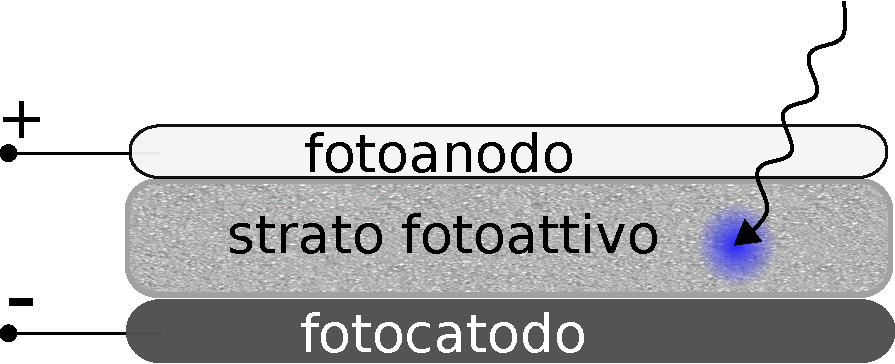
\includegraphics[width=.55\textwidth]{Immagini_Tesi/pv-schema1.pdf}}
\caption{\footnotesize{Uno schema generale di cella fotovoltaica.}
\label{fig:pv-schema1}}
\end{figure}

\section{Fotovoltaico}
Una cella fotovoltaica è un dispositivo atto a convertire energia luminosa in energia elettrica. Lo schema generale di una cella fotovoltaica è riportato in~\ref{fig:pv-schema1}.
Le funzioni, illustrate in~\ref{fig:livelli}, che devono essere svolte dai componenti di una cella sono:
\begin{enumerate}[label=\roman{*}.]
\item assorbimento della luce e fotogenerazione delle cariche,
\item trasporto delle cariche fino agli elettrodi,
\item trasferimento delle cariche sugli elettrodi.
\end{enumerate}

\begin{figure}
\centering{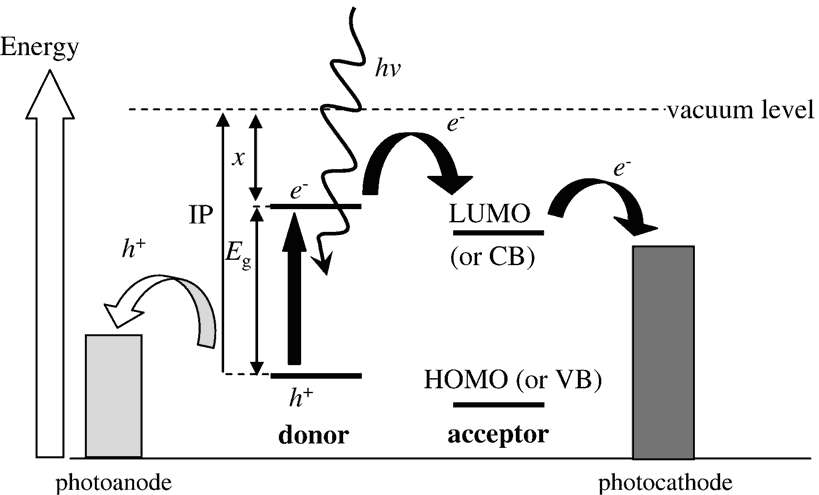
\includegraphics[width=.8\textwidth]{Immagini_Tesi/livelli.png}}
\caption{\footnotesize{Schema dei livelli energetici e della storia di una fotoeccitazione. Immagine tratta da \cite{fv-all}.}
\label{fig:livelli}}
\end{figure}
Le celle fotovoltaiche attualmente più diffuse sono basate sul silicio. 
Purtroppo è necessario utilizzare silicio ad elevati gradi di purezza (comunque inferiori al silicio per applicazioni elettroniche) e questo causa l'alto costo dei pannelli fotovoltaici classici.  
       
Per ovviare al problema del costo sono state sviluppate nuove combinazioni di materiali per applicazioni fotovoltaiche. 
Negli ultimi anni sono stati sviluppati materiali fotoattivi composti da nanoparticelle e polimeri semiconduttori. Le nanoparticelle utilizzate possono essere organiche o inorganiche ma in ogni caso si tratta di semiconduttori. Per i semiconduttori inorganici in forma di nanoparticelle si adotta il nome di \emph{quantum dots}\footnote{Quantum dot: materiale in cui i portatori di carica hanno zero gradi di libertà spaziale. Definizione data ma Mark Reed nel 1986.}. Inoltre queste nanoparticelle possono essere sferiche, a bacchetta o ramificate ( vedi~\ref{fig:NPs}).
          
I polimeri semiconduttori sono polimeri con una estesa coniugazione di doppi legami.        

Nei semiconduttori, a causa della loro struttura a bande illustrata in~\ref{fig:semicond-schema1}, non si ha presenza di cariche e lacune libere di condurre se il materiale si trova nello stato fondamentale. Una radiazione elettromagnetica con energia maggiore del \emph{band gap} può generare stati eccitati in cui si hanno elettroni nella banda di conduzione e lacune nella banda di valenza. Collegando questo semiconduttore con degli elettrodi metallici con livelli di Fermi\footnoteremember{Fermi}{{\descriptionlabel{Livello di Fermi}} allo zero assoluto coincide con l'energia di Fermi, ossia lo stato quantistico a più alta energia che risulta popolato allo zero assoluto. Invece a temperature maggiori è il potenziale chimico degli elettroni che compare nella distribuzione di Fermi-Dirac.} ad energia opportuna è possibile accumulare queste cariche ed ottenere una differenza di potenziale.
\begin{figure}
\centering{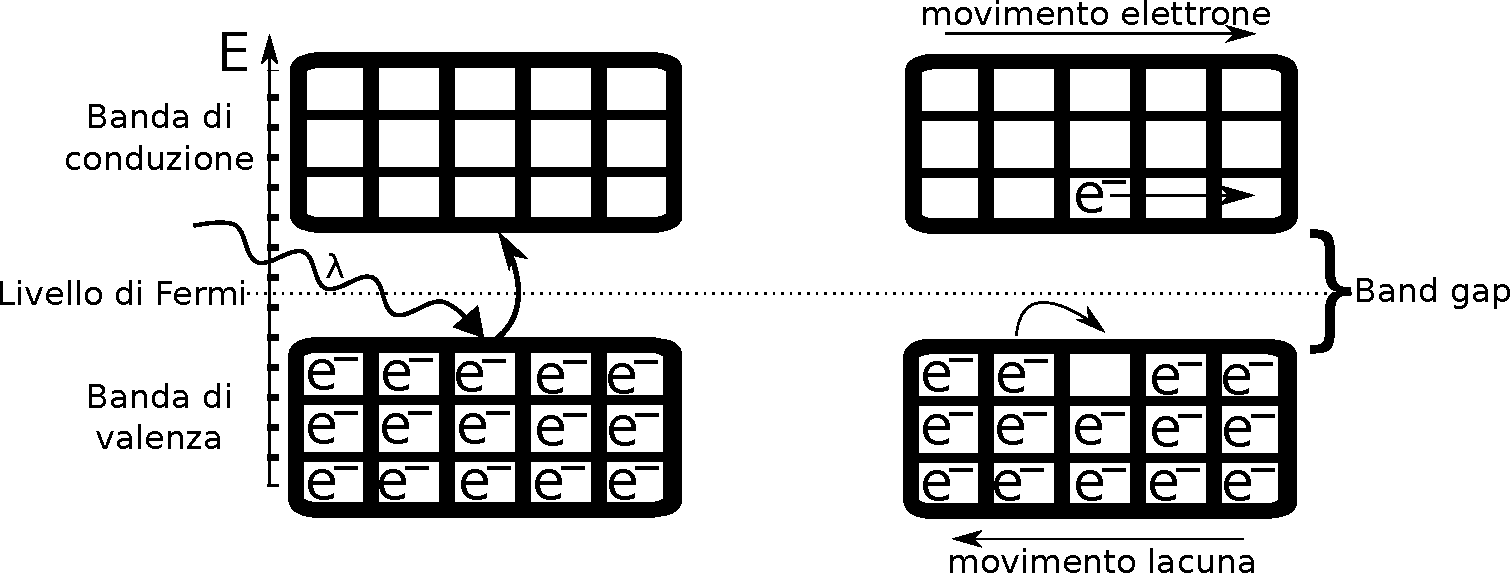
\includegraphics[width=.8\textwidth]{Immagini_Tesi/semicond-schema1.pdf}}
\caption{\footnotesize{Uno schema generale di sermiconduttore.}
\label{fig:semicond-schema1}}
\end{figure}

\subsection{Fotogenerazione di eccitoni}
Le radiazioni dello spettro solare possono venir assorbite da uno o da entrambi i semiconduttori presenti nello strato fotoattivo in funzione del loro \emph{band gap} (un materiale con \emph{band gap} minore assorbe una maggiore porzione dello spettro). Inoltre è possibile utilizzare un ``colorante'' inserito nello strato appositamente per fotogenerare cariche. Nel caso in studio sia le nanoparticelle che il polimero assorbono nel visibile e non verranno aggiunti coloranti. 
        

I polimeri coniugati hanno tipicamente una differenza LUMO - HOMO maggiore di 2~eV, corrispondente all'energia di un fotone con $\lambda=600$~nm. Con un tale \emph{band gap} i polimeri sono in grado di assorbire solo il 30\% della radiazione solare \cite{fv-eccit}. 
        

I fotoni assorbiti possono dare fotoeccitazioni diverse in dipendenza dalla loro energia che può essere maggiore o minore del \emph{band gap}. Nel primo caso l'energia è sufficiente a generare una lacuna ed un elettrone liberi ma le misurazioni danno per questo evento una resa quantica solamente di $\phi_{ch}\approx10\%$ \cite{pol-polarons}. Il restante 90\% e le radiazioni meno energetiche generano uno stato eccitato della materia detto eccitone. Questo è costituito da un elettrone e da una lacuna legati ossia che non hanno ricevuto energia sufficiente per separarsi. Recuperare l'energia contenuta negli eccitoni permetterebbe di aumentare molto l'efficienza energetica\footnoteremember{PCE}{{\descriptionlabel{Efficienza energetica (Power Conversion Efficiency PCE)}} rapporto tra la massima potenza in uscita e la potenza incidente in ingresso.} della cella fotovoltaica.
\subsection{Separazione delle cariche}
La separazione delle cariche che legate costituiscono l'eccitone è possibile se questo incontra una zona di forte campo elettrico \cite{fv-pcbm}. Questo si può generare all'interfaccia tra due materiali in cui si ha un accumulo di cariche. Questo accumulo si forma spontaneamente per mantenere l'uniformità spaziale del livello di Fermi \footnoterecall{Fermi} e per congiungere le bande di valenza e conduzione.
Il raggiungimento di questo equilibrio è illustrato in~\ref{fig:depletion_layer}.
\begin{figure}
\centering{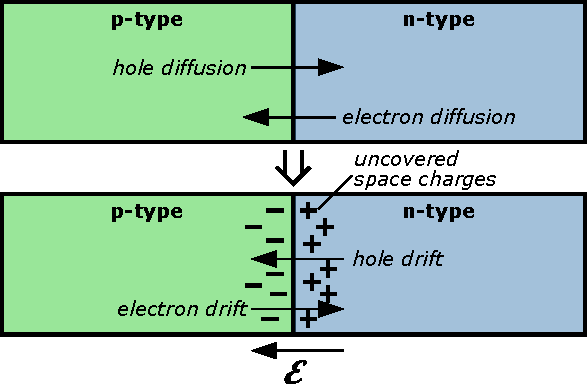
\includegraphics[width=.6\textwidth]{Immagini_Tesi/depletion_layer.pdf}}
\caption{\footnotesize{Sopra: giunzione $p-n$ prima della diffusione; sotto: dopo il raggiungimento dell'equilibrio. Immagine tratta da Wikimedia.}
\label{fig:depletion_layer}}
\end{figure}
\subsection{Trasporto delle cariche}
\label{sec:trasporto}
Una volta separate, le cariche devono essere trasportate fino agli elettrodi. Il movimento è indotto dal potenziale dei materiali utilizzati negli elettrodi come schematizzato in~\ref{fig:livelli}. Per limitare la ricombinazione tra cariche negative e lacune positive si utilizzano due materiali diversi per il trasporto. Questi possono essere gli stessi che costituiscono l'interfaccia, nel caso in studio il polimero semiconduttore e le nanoparticelle semiconduttrici. Per ottenere una buona conduzione si vuole una continuità all'interno di ciascun semiconduttore, ossia deve esistere un percorso di semiconduttore che connetta l'interfaccia interna al bordo dello strato fotoattivo. Nel caso della fase polimerica si deve considerare che le cariche non sono libere quanto in un semiconduttore inorganico, bensì deve aver luogo anche un trasporto intercatena. Questo trasporto viene reso più difficoltoso dalla presenza delle catene laterali alifatiche tipicamente presenti sul polimero e necessarie per rendere solubile il polimero stesso.
\subsection{Morfologia}
Un eccitone si propaga per brevi distanze, tipicamente 10nm in un semiconduttore organico \cite{fv-CdSe-OA}, prima di decadere radiativamente. Per avere una separazione efficace delle cariche è necessario che gli eccitoni incontrino una interfaccia nel loro breve tempo di vita. Le prime celle a polimeri erano costituite di due strati di polimero sovrapposti (morfologia \emph{bilayer}): uno per il trasporto degli elettroni ed uno per il trasporto delle lacune (vedi~\ref{fig:bilayer-bulk-heterojunction}).

\begin{figure}[!htb]
\centering{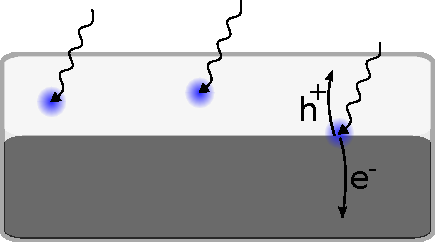
\includegraphics[width=.385\textwidth]{Immagini_Tesi/bilayer-eccitoni.pdf}
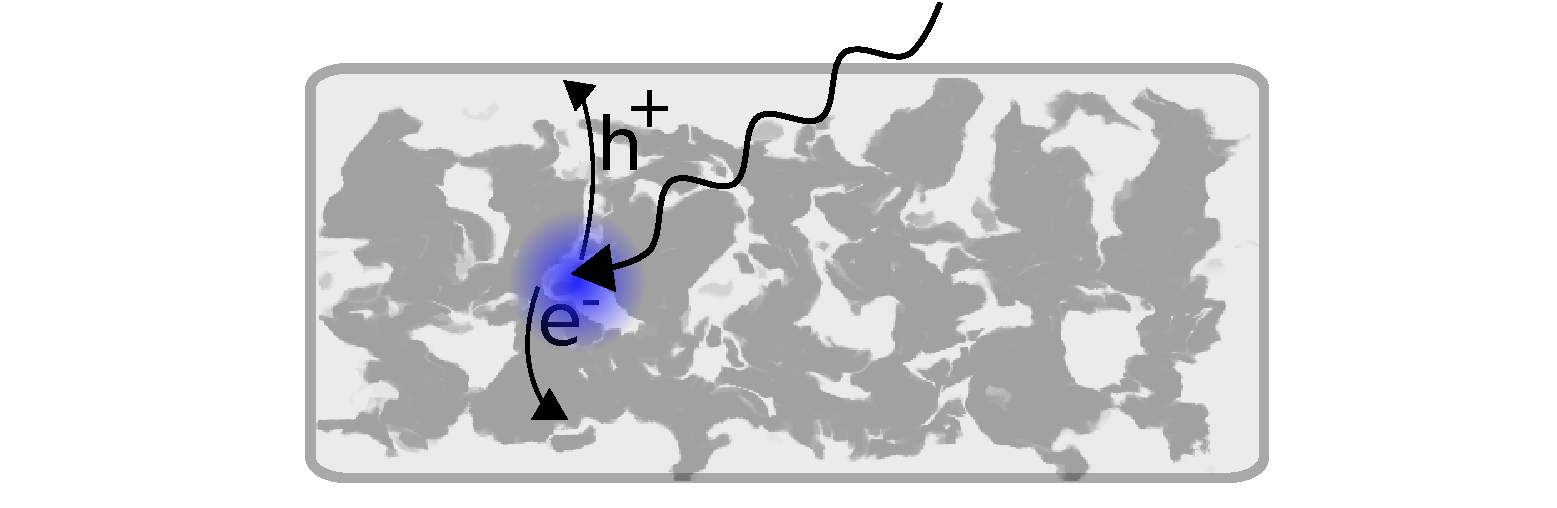
\includegraphics[width=.605\textwidth]{Immagini_Tesi/bulk-heterojunction-eccitoni.pdf}\\
\makebox{\parbox[b]{.385\textwidth}{\centering{(a)}}}
\makebox{\parbox[b]{.605\textwidth}{\centering{(b)}}}}
\caption{\footnotesize{Alcune morfologie: (a) \emph{bilayer}, (b) \emph{bulk heterojunction}. }}
\label{fig:bilayer-bulk-heterojunction}
\end{figure}
  

In queste celle la maggior parte degli eccitoni decadeva radiativamente prima di raggiungere l'interfaccia e di essere spezzati in cariche. Perciò una morfologia che può dare efficienze energetiche\footnoterecall{PCE} maggiori ha una interfaccia distribuita nello strato attivo: un \emph{bulk heterojunction}. Il \emph{bulk heterojunction} è illustrato in~\ref{fig:bilayer-bulk-heterojunction}-(b).
Il problema principale di una morfologia \emph{bulk heterojunction} si incontra nella sua formazione: i due semiconduttori non sono miscibili tra loro e tendono a separarsi dando estese aggregazioni come illustrato in~\ref{fig:interconnessi-allineati}-(a). Confrontandole con le nanoparticelle organiche, le inorganiche hanno una tendenza ad aggregarsi molto maggiore.
\setlength{\captionmargin}{.05\textwidth}  
\begin{figure}[!htb]
\centering{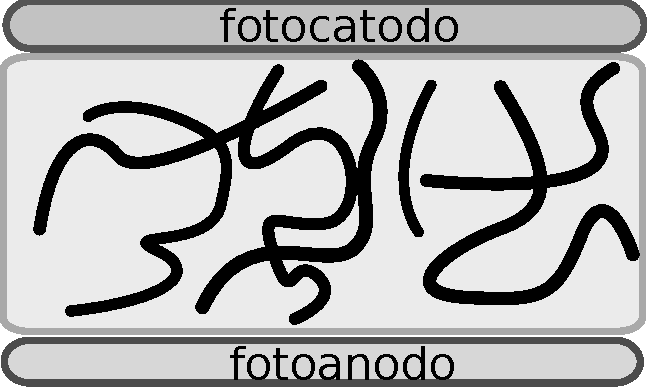
\includegraphics[width=.476\textwidth]{Immagini_Tesi/interconnessi_poco_aggregati.pdf}
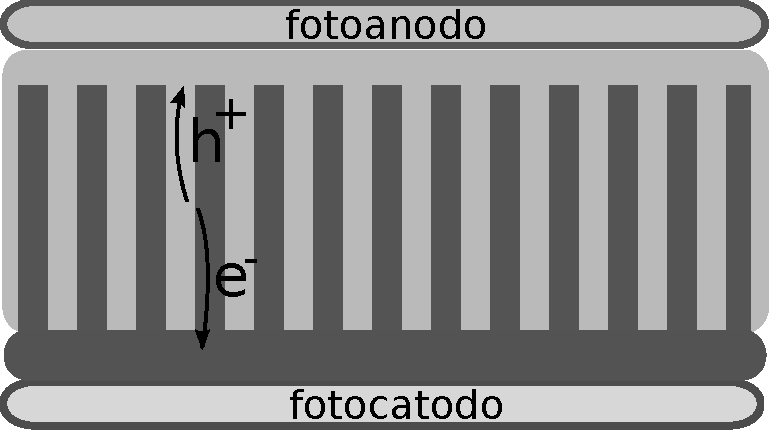
\includegraphics[width=.514\textwidth]{Immagini_Tesi/aggregati_allineati.pdf}\\
\makebox{\parbox[b]{.476\textwidth}{\centering{(a)}}}
\makebox{\parbox[b]{.514\textwidth}{\centering{(b)}}}}
\caption{\footnotesize{(a) La tendenza ad aggregarsi delle nanoparticelle produce sistemi con minore superficie di interfaccia. \\(b) La morfologia ideale per una cella solare \emph{bulk heterojunction}. }}
\label{fig:interconnessi-allineati}
\end{figure}
\setlength{\captionmargin}{.10\textwidth} 

Un possibile approccio volto ad aumentarne la miscibilità o comunque la dispersibilità in una matrice costituita dal polimero coniugato consiste nella modifica di una porzione del polimero coniugato introducendo funzionalità leganti nei confronti delle nanoparticelle. Questo verrà discusso nella Sottosezione~\ref{subsec:polimeri_cond}.

La morfologia ideale delle due fasi è costituita dalle fasi allineate verticalmente \cite{fv-morf-allineata} come illustrato in~\ref{fig:interconnessi-allineati}-(b). In questa struttura si minimizzano le ricombinazioni. La percolazione delle due fasi termina prima degli elettrodi per impedire la collezione di cariche di segno sbagliato sugli stessi.
      

Il problema principale consiste, come facilmente intuibile, nella difficoltà di ottenere tale morfologia con processi di fabbricazione o di autoassemblaggio.

\section{Caratteristiche dei materiali}

\subsection{Nanoparticelle}
\begin{figure}
\centering{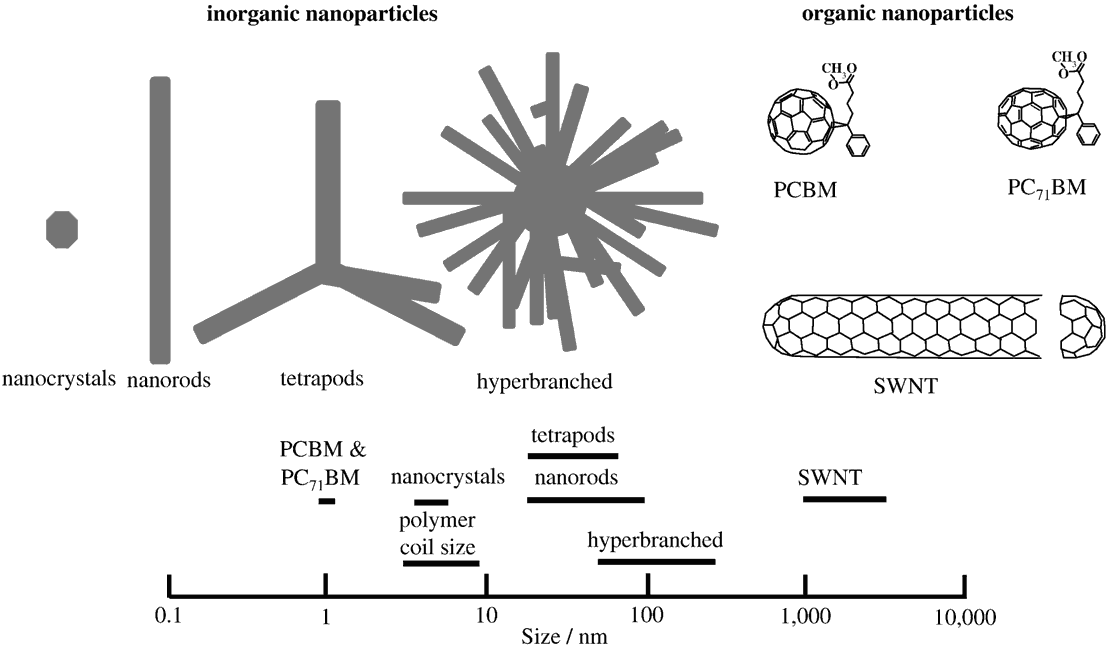
\includegraphics[width=.7\textwidth]{Immagini_Tesi/NPs2.png}}
\caption{\footnotesize{Esempi di nanoparticelle: a sinistra inorganiche, a destra organiche. Immagine tratta da \cite{fv-all}.}
\label{fig:NPs}}
\end{figure}
Le nanoparticelle possono essere semiconduttori organici o inorganici. In entrambi i casi vengono utilizzate come accettori e trasportatori di elettroni. Sia le organiche che le inorganiche possono avere forma sferica o più complessa ( vedi~\ref{fig:NPs} ). In questo lavoro verranno sintetizzate solo nanoparticelle inorganiche (nanocristalli) le quali presentano i seguenti vantaggi e svantaggi:
\begin{itemize}
 \item[\checkmark] i livelli energetici possono esser variati con la dimensione,
 \item[\checkmark] hanno alti coefficienti di assorbimento della luce,
 \item[\checkmark] hanno una mobilità elettronica più alta delle nanoparticelle organiche \cite{fv-CdSe-OA},
 \item[$\times$] le efficienze ottenibili sono in genere più basse a causa della maggiore aggregazione \cite{fv-all}, 
 \item[$\times$] l'uso dei metalli pesanti utilizzati è limitato per via della loro tossicità,
 \item[$\times$] hanno dimensioni maggiori delle nanoparticelle sferiche organiche (PCBM) perciò risulta una minore superficie interfacciale \cite{fv-all}.
\end{itemize}
La forma delle nanoparticelle sarà sferica per semplicità di sintesi. 
In letteratura si trovano molti materiali semiconduttori utilizzabili per i nostri scopi: TiO$_2$, ZnO, PbS, CdSe, CdTe, CuInSe$_2$, CuInS$_2$, CdS, PbSe, GaAs \ldots In questo lavoro si utilizzeranno nanocristalli sferici di CdSe. Per questo semiconduttore la letteratura riporta le efficienze energetiche più alte \cite{fv-all}. Inoltre è possibile la sintesi di nanofili e di strutture ramificate di CdSe per ulteriori sviluppi di questi sistemi verso efficienze più elevate. 
\subsection{Polimeri semiconduttori}

\label{subsec:polimeri_cond}
I polimeri semiconduttori sono molecole con una estesa coniugazione di doppi legami e/o sistemi aromatici. Hanno la funzione sia di assorbire la luce sia di donare elettroni e di trasportare lacune. 
        
I polimeri semiconduttori più usati per applicazioni nel fotovoltaico organico o ibrido sono idrofobici e sono elencati in~\ref{fig:polimericonduttori}.
\setlength{\captionmargin}{-.05\textwidth}
\begin{figure}
\centering{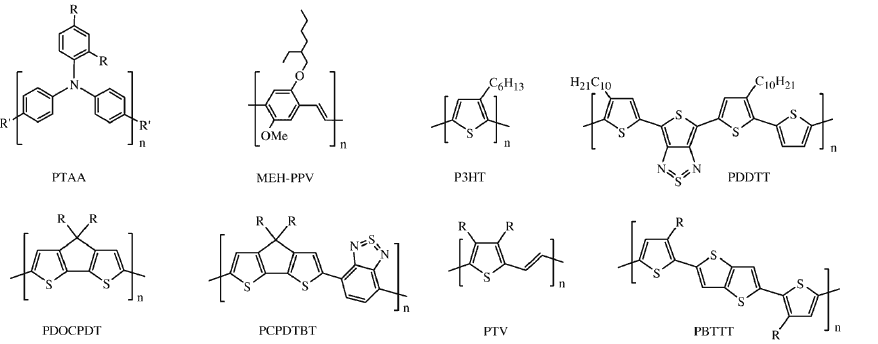
\includegraphics[width=.9\textwidth]{Immagini_Tesi/polimericonduttori2.png}}
\caption{\footnotesize{Struttura dei polimeri semiconduttori utilizzati nelle celle fotovoltaiche. PTAA: poli(triarilammina); MEH-PPV: poli(2-metossi-5-etilesilossifenilene vinilene); P3HT: poli(3-esiltiofene); PDDTT: poly[5,7-bis(4-decanyl-2-thienyl)thieno[3,4-b]diathiazole-thiophene-2,5)]; PDOCPDT: poly[2,5-(7,7-dioctyl)-cyclopentadithiophene]; PCPDTBT: poly[2,6-(4,4-bis-(2-ethyhexyl)-4H-cyclopenta[2,1-b;3,4-b′]-dithiophene)-alt-4,7-(2,1,3-benzothiadiazole)]; PTV: poli(tienilene vinilene); PBTTT: poly[2,5-bis(3-alkylthiophen-2-yl)thieno[3,2-b]thiophene)].
Immagine tratta da \cite{fv-all}}
\label{fig:polimericonduttori}}
\end{figure}
        
In un polimero coniugato il \emph{band gap} è la differenza LUMO - HOMO\@. Questi corrispondono rispettivamente alla banda di conduzione e di valenza. 

Solitamente la separazione è maggiore di 2~eV, perciò l'energia termica a temperatura ambiente non è sufficiente a popolare il LUMO ed il polimero risulta un semiconduttore.
Se a questo viene donato o sottratto un elettrone allora diventerà conduttore (vedi~\ref{fig:semicond-schema1}). Ciò avviene durante la separazione degli eccitoni formati con l'assorbimento dei fotoni. 
\setlength{\captionmargin}{.0\textwidth}  

\begin{wrapfigure}{r}{0.50\textwidth}
\begin{center}
    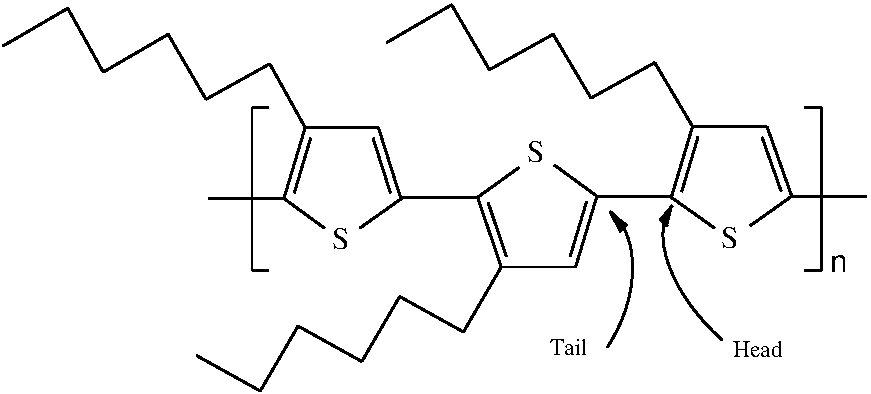
\includegraphics[width=1\textwidth]{Immagini_Tesi/p3ht-htht.pdf}
  \end{center}
  \vspace{-5pt}\footnotesize{\caption{Poli(3-esiltiofene) regioregolare \emph{head-tail-head-tail}.\label{fig:p3ht-htht}}}
\end{wrapfigure}
\setlength{\captionmargin}{.10\textwidth}  
      
La differenza LUMO - HOMO dipende dal monomero e diminuisce con la lunghezza di coniugazione fino al raggiungimento di 15-20 unità monomeriche, oltre la quale si stabilizza. Perché questa coniugazione sia presente è necessario che il polimero sia planare. 


La sua planarità (ed il trasporto intercatena, vedi Sottosezione~\ref{sec:trasporto}) è disturbata dalla repulsione tra le catene laterali alifatiche necessarie per rendere il polimero solubile in solventi organici e quindi lavorabile, tipicamente per deposizione su un supporto tramite \emph{spin coating}. 


Questa interazione può essere minimizzata nel caso di polimeri con unità ripetenti a struttura asimmetrica sintetizzando un polimero regioregolare \emph{head-tail-head-tail}\label{regio-htht}, vedi~\ref{fig:p3ht-htht}. 
 
Il polimero che verrà sintetizzato in questa tesi è il poli(3-esiltiofene). Questa scelta è motivata dal fatto che i livelli energetici del CdSe sono adatti ad essere accoppiati con quelli del politiofene: la differenza energetica tra il LUMO del polimero donatore e la banda di conduzione delle nanoparticelle accettrici (vedi~\ref{fig:livelli}) deve essere non troppo piccola ma nemmeno troppo grande per evitare la popolazione di stati di tripletto del polimero. Inoltre è stato riportato in letteratura che la lunghezza massima di coniugazione raggiunge le 20 unità monomeriche \cite{pol-pti-lunghezza}. 


\section{Scopo del tirocinio}

Lo scopo di questo tirocinio è la realizzazione di nuovi materiali ibridi potenzialmente utilizzabili per lo strato fotoattivo di celle fotovoltaiche orgaiche di tipo \emph{bulk heterojunction}. In particolare verranno preparati nanocristalli di CdSe modificati con poli(3-esiltiofene). 

Il poli(3-esiltiofene) non verrà utilizzato tal quale per disperdere le nanoparticelle, bensì verrà funzionalizzato con gruppi leganti nei confronti del CdSe allo scopo di contrastare la tendenza delle \emph{NPs}\footnoteremember{NPs}{{\descriptionlabel{NPs}} nanoparticelle} all'aggregazione ed alla separazione delle fasi.

Come viene schematizzato in~\ref{fig:leganti} i gruppi leganti possono essere inseriti in varie posizioni sul polimero: nelle catene laterali, su entrambe le terminazioni, in un blocco di polimero legante non coniugato o solamente su una delle due terminazioni.
\begin{figure}
\centering{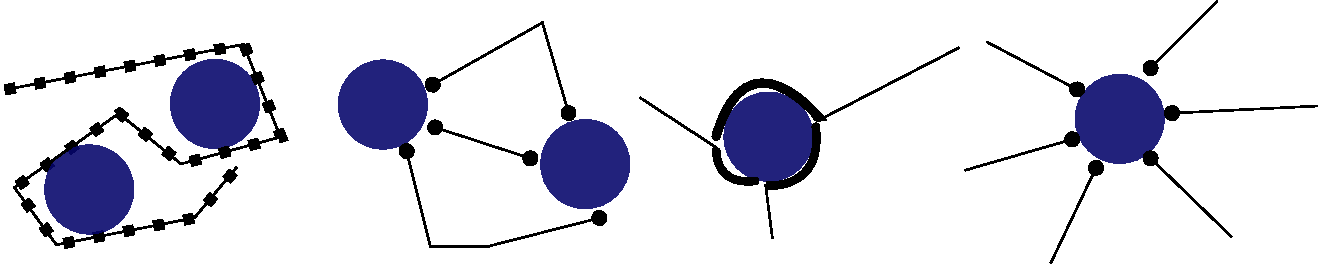
\includegraphics[width=.8\textwidth]{Immagini_Tesi/leganti.pdf}}
\caption{\footnotesize{Le posizioni in cui possono essere inseriti gruppi leganti sul polimero semiconduttore.}
\label{fig:leganti}}
\end{figure}
In questo lavoro è stata presa in considerazione l'ultima di queste possibilità, ossia la singola terminazione legante. Infatti le prime due possibilità sono da escludersi perché porterebbero alla formazione di materiali reticolati non plastici (la plasticità è uno dei punti di forza del fotovoltaico organico ed ibrido organico-inorganico). La terza opzione è utilizzabile ma inserisce nell'interfaccia polimero-nanoparticella un secondo tipo di polimero che rischia di agire da isolante.

Tra i molti gruppi leganti riportati in letteratura per il CdSe ( tioli, ammine, acidi carbossilici, acidi fosfonici, piridine sostituite in para ed altri ) in questo lavoro di tesi verrà realizzata per la prima volta una miscela NPs\footnoterecall{NPs} di CdSe - politiofene monoterminato con un gruppo fosfonico. Come si può osservare nella~\ref{fig:pol-finale} l'altra terminazione del polimero sarà un gruppo allile.
\begin{figure}
\centering{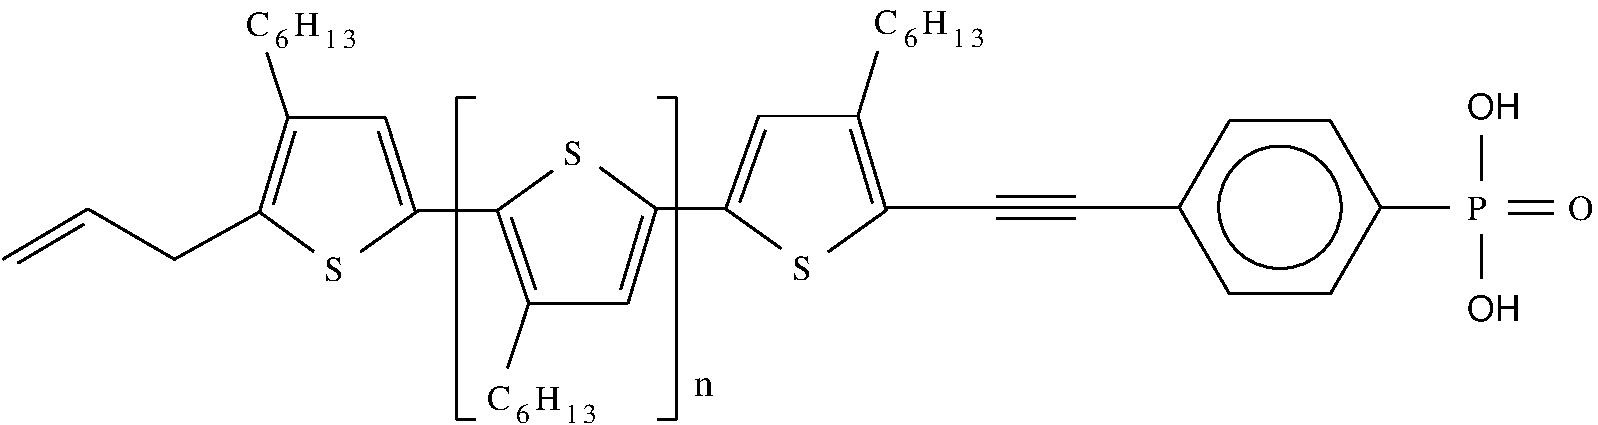
\includegraphics[width=1\textwidth]{Immagini_Tesi/pol-finale.pdf}}
\caption{\footnotesize{Il polimero sintetizzato completo di terminazione legante.}
\label{fig:pol-finale}}
\end{figure}

%%%%%%%%%%%%%%%%%%%%%% Capitolo 2 %%%%%%%%%%%%%%%%%%%%%%
\chapter{Sintesi dei materiali}

\section{Sintesi di \emph{quantum dots} di CdSe}
La sintesi di nanocristalli sferici di CdSe è stata eseguita seguendo la procedura messa a punto da Peng \cite{qd-CdSe-CdO}.
Si tratta di una sintesi in micelle inverse
\footnoteremember{micelle-inverse}{{\descriptionlabel{Sintesi in micelle inverse}} sintesi in cui la nanoparticella si forma in una zona polare separata dall'ambiente apolare tramite leganti con code apolari.} 
che utilizza CdO e polvere di selenio. L'utilizzo di micelle inverse\footnoterecall{micelle-inverse} è un metodo di sintesi semplice ed economico che permette un buon controllo della dimensione finale delle particelle e ne impedisce l'aggregazione passivandone la superficie. In letteratura si trovano molte altre procedure di sintesi che differiscono sostanzialmente per le fonti di cadmio e di selenio \cite{qd-CdSe-Cd,qd-CdSe-CdCl2}. Questa via ha come principale vantaggio l'impiego di una sorgente di cadmio non volatile e perciò più sicura rispetto alla migliore alternativa sintetica che comporta l'impiego di dimetilcadmio, volatile, tossico, sensibile all'aria ed esplosivo.

I leganti utilizzati per formare le micelle sono stati tri-{\itshape n}-ottilfosfina ossido (d'ora in poi TOPO) ed acido {\itshape n}-tetradecilfosfonico (d'ora in poi TDPA). Il secondo è un legante di superficie più affine al CdSe rispetto al primo \cite{lig-CdSe-P} ma verrà comunque sostituito nei passaggi di scambio di leganti (Sezione~\ref{sec:leganti}). 

La procedura messa a punto da Peng \cite{qd-CdSe-CdO} prevede di disperdere il CdO nei due leganti e la polvere di selenio in triottilfosfina (d'ora in poi TOP). Dopo aver scaldato e dissolto il CdO vi è stato iniettato rapidamente il Se in TOP\@. Il tutto è stato tenuto a 270°C per 5 minuti. Tutta la procedura è stata svolta in atmosfera di argon e proteggendo il pallone dalla luce. Le nanoparticelle ottenute sono state purificate precipitandole più volte in metanolo disareato per eliminare il TOPO non legato ed il TOP\@. Una volta seccate sotto flusso di azoto sono state ridissolte in toluene e filtrata la soluzione. Le caratterizzazioni effettuate (DLS
\footnoteremember{DLS}{{\descriptionlabel{DLS}} Dynamic Light Scattering, strumento per misurare il diametro idrodinamico di particelle disperse.}
, UV-vis\footnote{La lunghezza d'onda a cui si osserva il primo picco di assorbimento eccitonico può essere utilizzata per determinare il diametro delle NPs di CdSe utilizzando la formula empirica riportata a pagina \pageref{eq:diametro}}
, fotoluminescenza) hanno indicato un diametro di 2.1 - 2.9~nm. La caratterizzazione $^1$H-NMR e $^{31}$P $\{^1H\}$ NMR ha permesso di verificare la presenza dei 2 leganti di superficie.

\section[Sintesi di poli(3-esiltiofene) regioregolare terminato allile/Br]{Sintesi di poli(3-esiltiofene) regioregolare terminato asimmetricamente allile/Br}

La sintesi di poli(3-alchiltiofene) regioregolare può esser effettuata seguendo 3 schemi: metodo McCullough \cite{pol-McCullough}, metodo Rieke \cite{pol-rieke}, Grignard metatesi \cite{pol-grim}. Per quest'ultimo metodo è riportata in letteratura \cite{pol-p3ht-end} la possibilità di sintetizzare un polimero asimmetricamente terminato.
La procedura sintetica seguita per la sintesi di poli(3-esiltiofene) regioregolare terminato asimmetricamente allile/Br è stata sviluppata da Jeffries-El \etal \cite{pol-p3ht-end} e si tratta di una metatesi Grignard. Per questa procedura è riportata in letteratura una cinetica di polimerizzazione quasi vivente \cite{pol-grim-living}. Dato il carattere vivente (discusso più in basso) è possibile ottenere poli(3-esiltiofene) con bassa polidispersità\footnote{{\descriptionlabel{Polidispersità (PDI polydispersity index)}} è una misura della uniformità dei pesi molecolari delle catene polimeriche. Si esprime come rapporto tra la massa molare media pesata e massa media numerica del polimero.}. 

La sintesi avviene in 3 stadi: preparazione del monomero attivo, crescita del polimero, attacco del gruppo di terminazione allile.


\begin{figure}
\centering{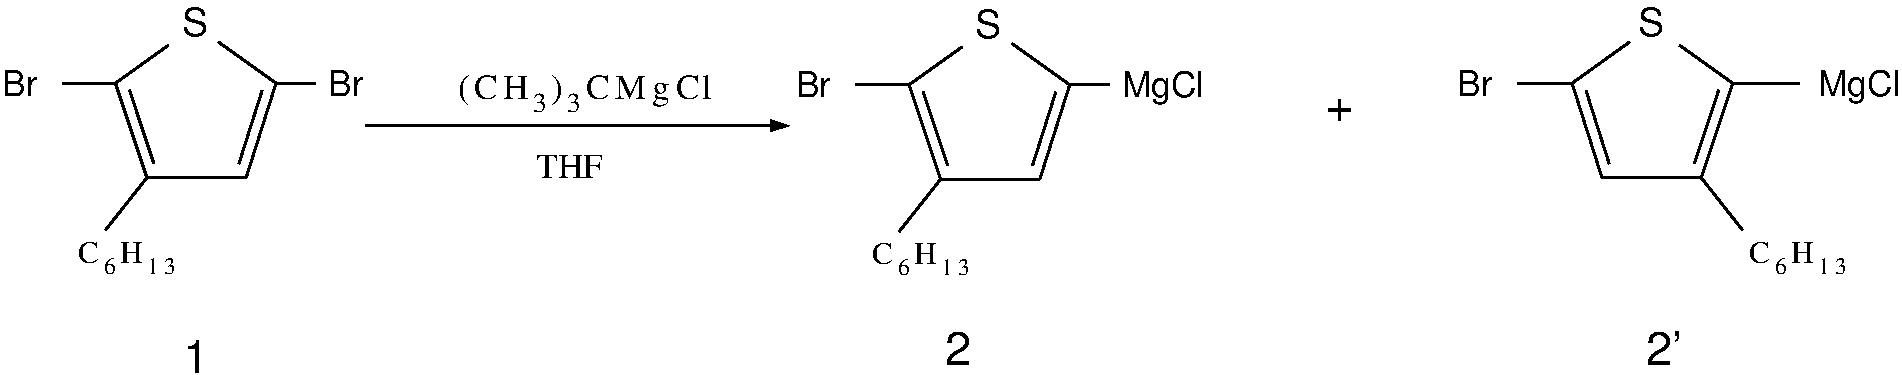
\includegraphics[width=.7\textwidth]{Immagini_Tesi/monomero-grignard.pdf}}
\caption{\footnotesize{Il monomero viene reso un reattivo di Grignard tramite una reazione di metatesi (doppio scambio).}
\label{fig:monomero-grignard}}
\end{figure}
Il monomero 2,5-dibromo-3-esiltiofene è stato trattato con 1 equivalente di \tBu magnesio cloruro e si sono ottenuti i 2 monomeri illustrati in~\ref{fig:monomero-grignard} tramite una reazione di doppio scambio denominata di metatesi Grignard. Nell'articolo di Iovu \etal \cite{pol-grim-living} è riportato il rapporto tra i due prodotti {\bf 2}:{\bf 2'}~=~da~85:15~a~75:25; inoltre nello stesso articolo viene riportato che il prodotto {\bf 2'} non viene consumato dalla polimerizzazione.

Successivamente è stato aggiunto il catalizzatore a base di Nickel: 1,3-bis(difenilfosfino) propano nickel(II) cloruro per avviare la polimerizzazione. 
Uno dei meccanismi proposti è illustrato in~\ref{fig:pol-polimerizz}.
\begin{figure}
\centering{
\includegraphics[width=.8\textwidth]{Immagini_Tesi/pol-polimerizz.png}}
\caption{\footnotesize{Il meccanismo proposto per la polimerizzazione GRIM del poli(3-alchiltiofene). Immagine tratta da \cite{pol-grim-living}.}
\label{fig:pol-polimerizz}}
\end{figure}
Il primo stadio consiste nello scambio tra i due anioni \ce{Cl-} e due formali anioni derivanti dal Grignard del monomero. Quindi con una eliminazione riduttiva si ha la formazione di un dimero \emph{tail-tail}\label{tail-tail}. Dopo la formazione del dimero il catalizzatore vi resta legato in una coppia associata da cui poi ha il via la polimerizzazione vera e propria. 
Lo stadio lento del ciclo di polimerizzazione, che causa il carattere quasi vivente, è la transmetallazione. 

Infine, come illustrato in~\ref{fig:grim-end}, si è aggiunto allilmagnesio bromuro per terminare un solo capo della catena polimerica con un gruppo allile. Non avviene il doppio attacco ad entrambe le terminazioni perché si ha formazione di una coppia associata tra il catalizzatore ed il primo gruppo terminante inserito. Nell'articolo \cite{pol-p3ht-end} da cui è tratta questa procedura vengono riportati anche altri reattivi di Grignard con cui è possibile ottenere una singola terminazione. Alcuni di questi reattivi sono stati testati in precedenti lavori del nostro gruppo e la migliore resa è stata ottenuta utilizzando allilmagnesio bromuro.

\begin{figure}
\centering{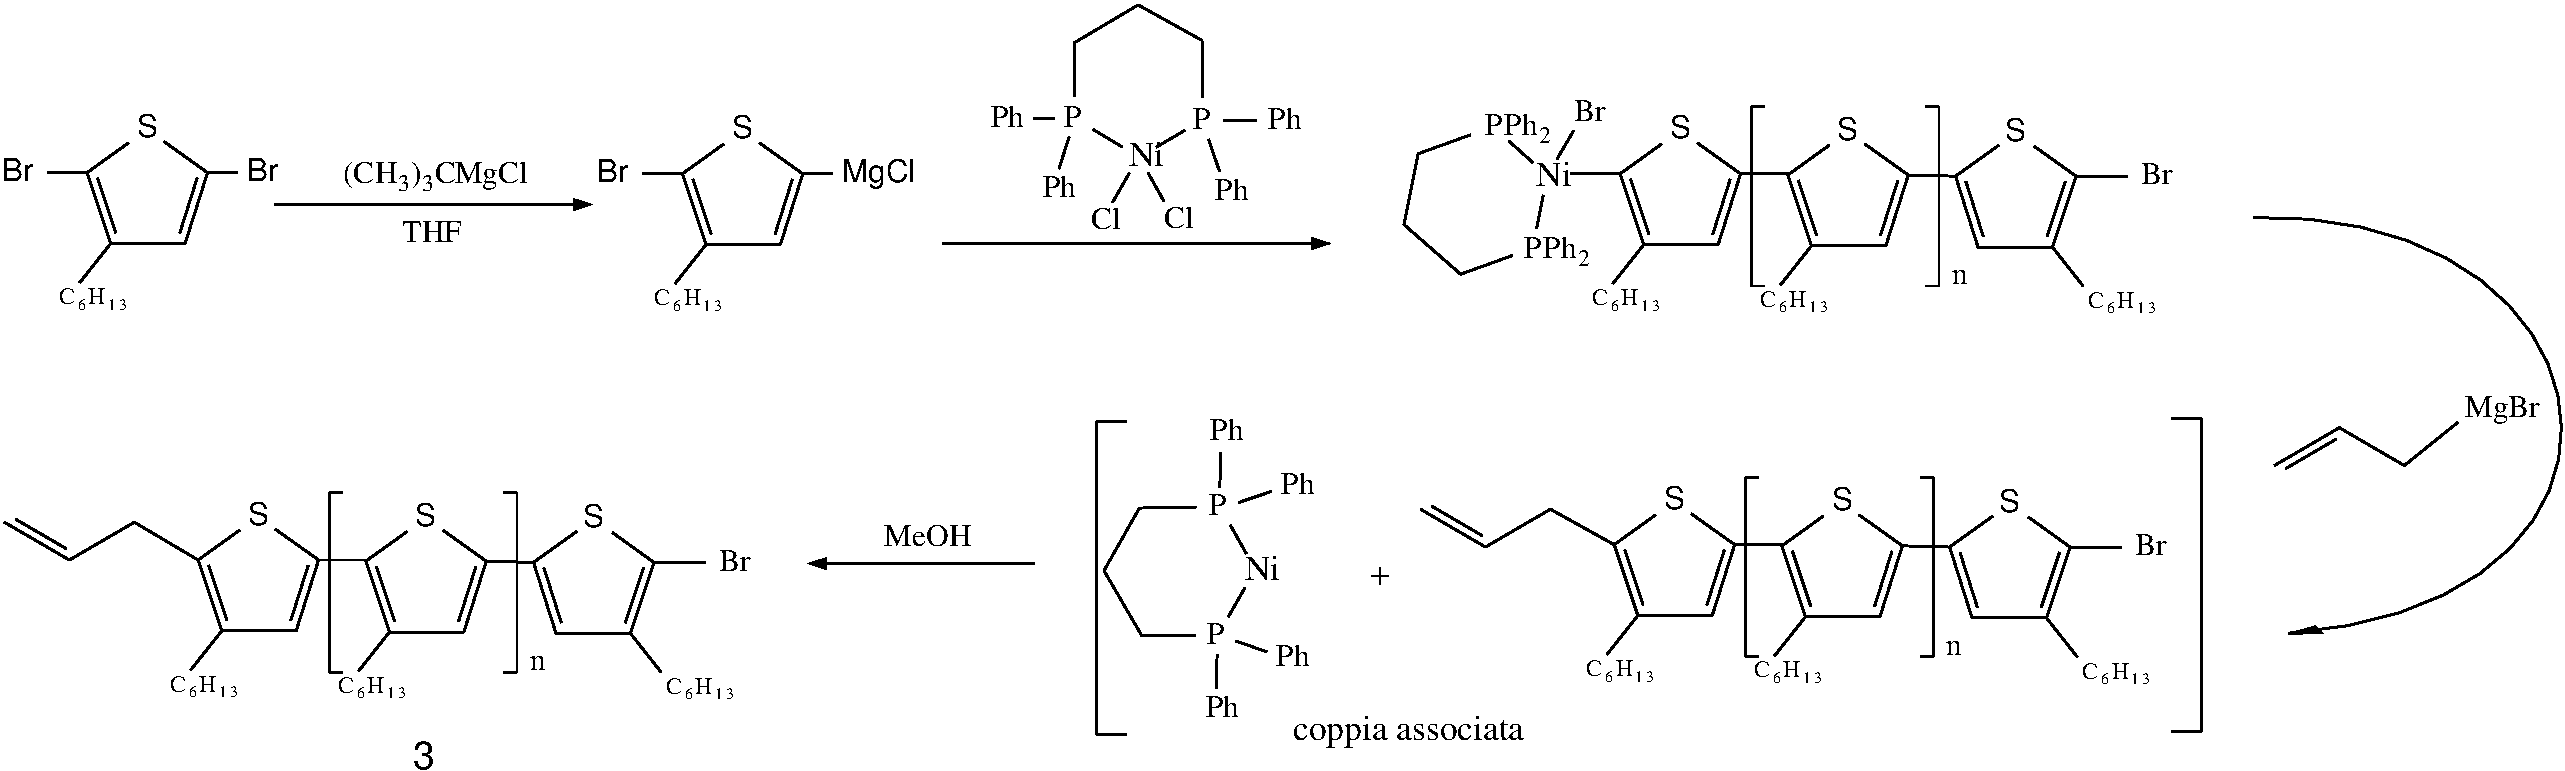
\includegraphics[width=.99\textwidth]{Immagini_Tesi/grim-end.pdf}}
\caption{\footnotesize{Lo schema generale della polimerizzazione e della terminazione.}
\label{fig:grim-end}}
\end{figure}
Il prodotto {\bf 3} è stato purificato con metanolo e {\itshape n}-esano ed infine raccolto in cloroformio e seccato. 

La caratterizzazione $^1$H-NMR ha permesso di verificare la regioregolarità, la terminazione asimmetrica e di stimare la lunghezza del polimero.
\section{Sintesi di poli(3-esiltiofene) terminato allile/legante fosfonico}
In questa sezione si espone la modifica del prodotto \n{3} della sezione precedente al fine di ottenere un gruppo legante su una delle due terminazioni del polimero. L'attacco avverrà sulla terminazione presentante un bromo sfruttando la sua reattività in un \emph{coupling} di Sonogashira. Invece la terminazione allilica resterà inalterata e presente sul polimero finale \n{7}.

 Si ha a disposizione la molecola dietil (4-bromofenil)fosfonato ({\bf 4}) precedentemente sintetizzata che presenta un gruppo fosfonico protetto da etili. 

La sintesi si può dividere in 3 fasi: modifica del legante ed attacco al polimero entrambi con un \emph{coupling} di Sonogashira ed infine deprotezione del gruppo fosfonico.

Come illustrato in~\ref{fig:legante} al legante è stato aggiunto tramite un \emph{coupling} di Sonogashira un gruppo alchinico monoprotetto con il gruppo trimetilsilile per non dare ulteriore accoppiamento. 
\begin{figure}
\centering{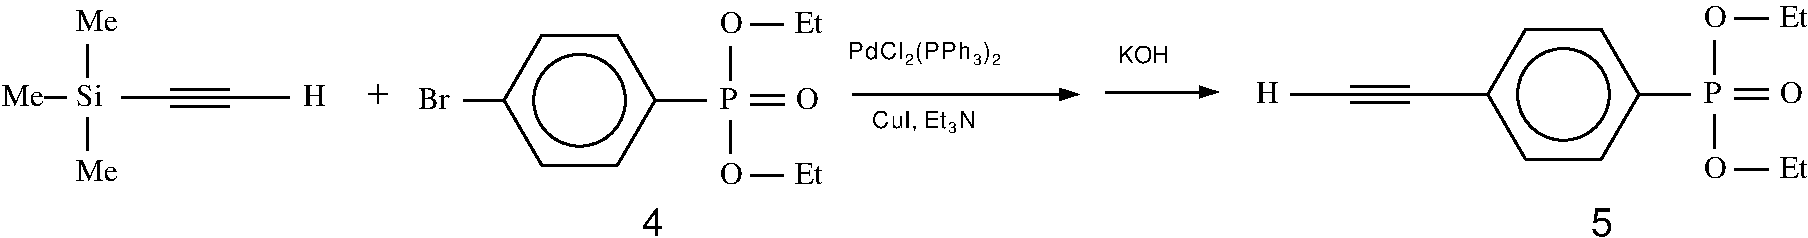
\includegraphics[width=1\textwidth]{Immagini_Tesi/legante.pdf}}
\caption{\footnotesize{Schema della modifica e della deprotezione del legante.}
\label{fig:legante}}
\end{figure}

Quindi la protezione è stata rimossa con KOH e, dopo purificazione su colonna, è stato eseguito un secondo \emph{coupling} di Sonogashira tra il legante \n{5} ed il polimero \n{3} terminato allile/bromo come illustrato in~\ref{fig:p3ht-legante}. Infine è stata rimossa la protezione del gruppo fosfonico utilizzando trimetilbromosilano per ottenere il polimero finale \n{7}. 
\begin{figure}
\centering{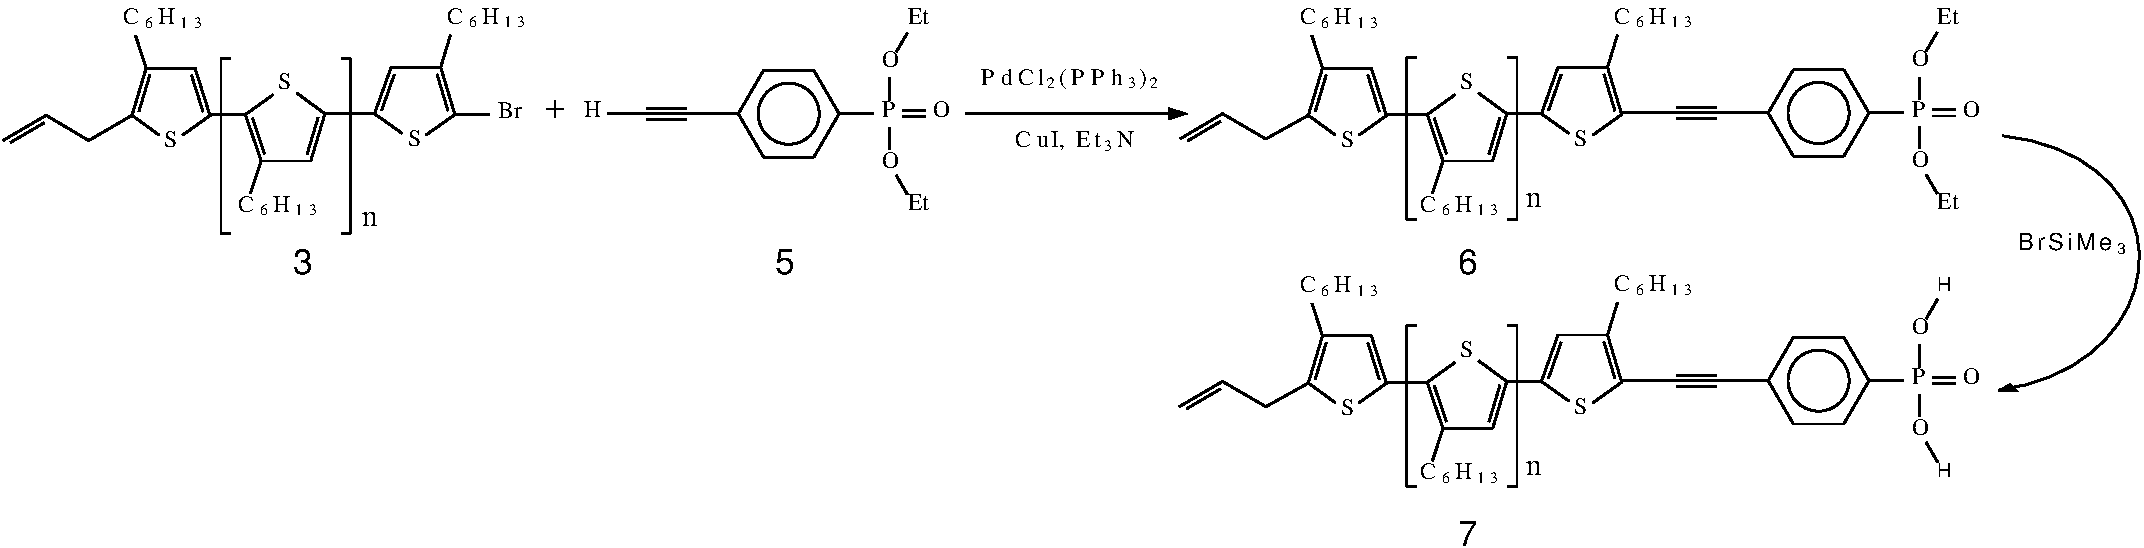
\includegraphics[width=1.1\textwidth]{Immagini_Tesi/p3ht-legante.pdf}}
\caption{\footnotesize{Schema del \emph{coupling} di Sonogashira tra il legante \n{5} ed il polimero \n{3} con successiva deprotezione a \n{7}.}
\label{fig:p3ht-legante}}
\end{figure}

La caratterizzazione $^1$H-NMR del polimero finale, costituito da una catena oligomerica idrofoba con una 
terminazione idrofila, non ha consentito di evidenziare la presenza dei segnali relativi alla terminazione legante. Questo fatto inatteso si ritiene sia dovuto non alla mancata funzionalizzazione ma piuttosto alla formazione di strutture micellari, cioè di sistemi quasi solidi non analizzabili con tecniche convenzionali di NMR in soluzione~\cite{lig-micelle-nmr2}. 

\section{Scambio di leganti}
\label{sec:leganti}
Allo scopo di ottenere i \emph{quantum dots} passivati almeno in parte dal polimero sintetizzato \n{7} è necessario effettuare uno scambio di leganti di superficie. Purtroppo il gruppo legante presente su {\bf 7} ha una affinità per la superficie delle NPs comparabile con l'affinità del TOPO e del TDPA\@. Dunque uno scambio diretto avrebbe una resa limitata. È possibile ovviare a questo problema effettuando due scambi di leganti: la sostituzione di TOPO con un legante blando come la piridina e successivamente lo scambio della piridina col polimero \n{7}.

 Si prevede che la maggior parte del TOPO (una trialchil fosfina ossido) venga sostituito dalla piridina, mentre il TDPA (un acido fosfonico) essendo più affine alla superficie \cite{lig-CdSe-P} dovrebbe esser rimosso più difficilmente. 
Questo primo scambio di leganti viene eseguito semplicemente sciogliendo le NPs in piridina e scaldando per tempo sufficiente. La procedura è stata sviluppata da Peng \etal \cite{lig-pyridine}. Le nuove nanoparticelle parzialmente passivate con piridina sono risultate, al contrario di quelle stabilizzate solo dai leganti fosforati aventi lunghe catene alchiliche, solubili in metanolo ed insolubili in {\itshape n}-esano. La procedura di sostituzione e purificazione è consistita in diversi cicli di dissoluzione in piridina e precipitazione in {\itshape n}-esano.

Nel secondo scambio, in cui si vuole ottenere le NPs di CdSe passivate col polimero {\bf 7}, è necessario utilizzare un solvente che solvati entrambi i precursori, ossia sia le particelle passivate con TOPO, TDPA e piridina che il politiofene con funzionalità terminale fosfonica, come tetraidrofurano o cloroformio. Si è scelto di utilizzare come solvente il cloroformio, quindi vi sono stati disciolti uguali pesi di polimero e di \emph{quantum dots} e si è lasciato procedere lo scambio di leganti a temperatura ambiente. Il rapporto in peso di polimero e nanoparticella è stato scelto sulla base delle indicazioni di letteratura scientifica relative ai sistemi oggetto di studio in grado di dare l'efficienza energetica più elevata~\cite{qd-ratio-CdSe_vs_pol}.



%%%%%%%%%%%%%%%%%%%%%% Capitolo 3 %%%%%%%%%%%%%%%%%%%%%%
%%%%%%%% Capitolo3 %%%%%%%%
\chapter{Caratterizzazione dei materiali}
\label{chap:risultati}

\section[Quantum Dots]{\emph{Quantum Dots}}
 Qui di seguito sono riportati i risultati delle caratterizzazioni FT-IR, UV-vis, fotoluminescenza, DLS (\emph{Dynamic Light Scattering}), 
 $^{31}$P-NMR e TEM eseguite sulle nanoparticelle di CdSe passivate con leganti TOPO (tri-ottilfosfina ossido) e TDPA (acido 1-tetradecilfosfonico).

{
Confrontando gli spettri FT-IR in~\ref{fig:CdSe-TOPO_TDPA-IR-TOPO_TDPA} possiamo osservare che il debole picco dello \emph{stretching} P=O a 1125~cm$^{-1}$ si sposta a 1101~cm$^{-1}$ in presenza delle nanoparticelle, questo può essere attribuito alla coordinazione del gruppo fosfonico al CdSe tramite l'ossigeno P=O  \cite{lig-CdSe-caratt}}. 

\begin{figure}
\centering{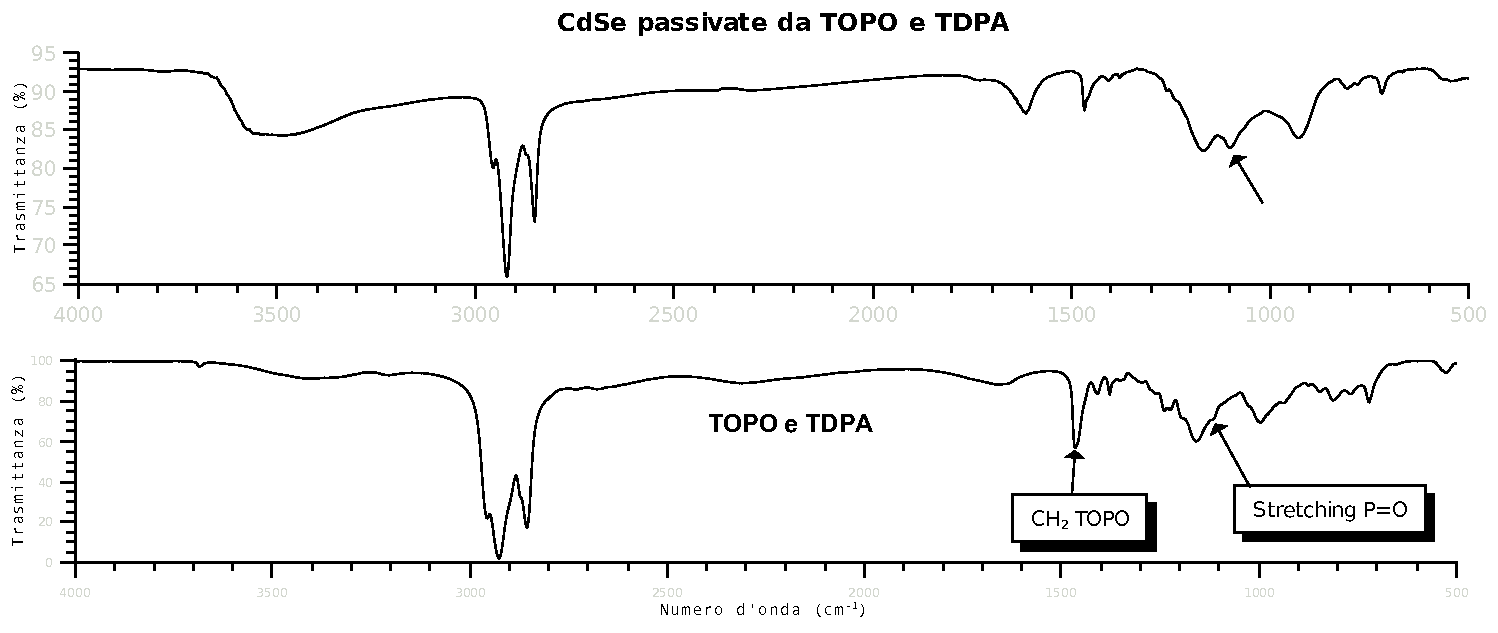
\includegraphics[width=.93\textwidth]{Immagini_Tesi/caratterizzazione/CdSe-TOPO_TDPA-IR-TOPO_TDPA.pdf}}
\caption{\footnotesize{In alto spettro FT-IR di NPs passivate con TOPO e TDPA\@. In basso spettro FT-IR di TOPO e TDPA puri.}
\label{fig:CdSe-TOPO_TDPA-IR-TOPO_TDPA}}
\end{figure}

\begin{figure}[!htb]
\centering{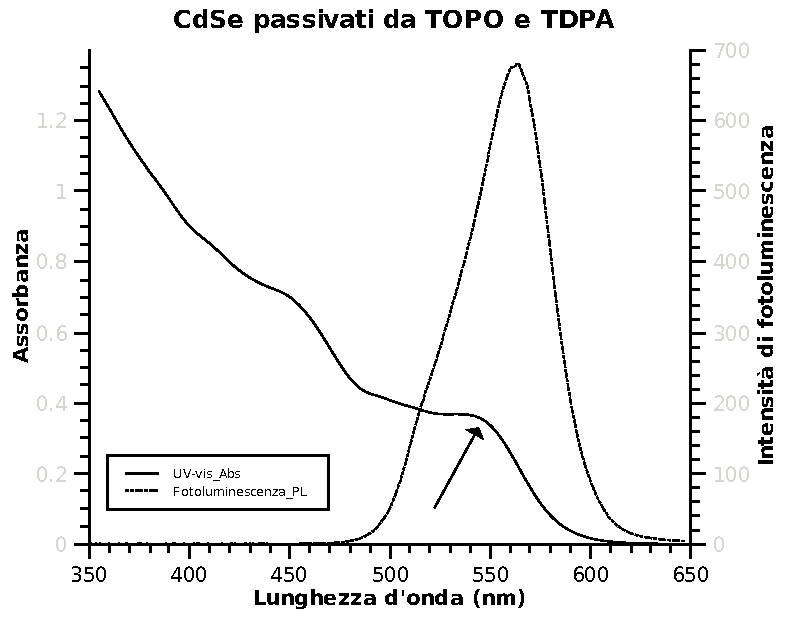
\includegraphics[width=.495\textwidth]{Immagini_Tesi/caratterizzazione/CdSe-TOPO_TDPA-in_toluene-UV_PL.pdf}
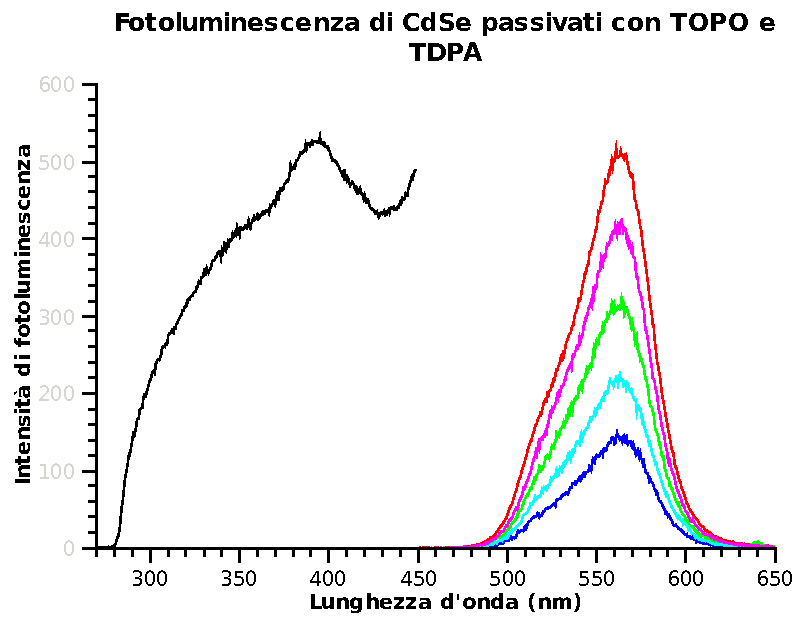
\includegraphics[width=.495\textwidth]{Immagini_Tesi/caratterizzazione/CdSe-TOPO_TDPA-movimentobanda-PL.pdf}\\
\makebox{\parbox[b]{.495\textwidth}{\centering{(a)}}}
\makebox{\parbox[b]{.495\textwidth}{\centering{(b)}}}}
\caption{\footnotesize{(a) Spettro UV-vis (---) e fotoluminescenza (- - -) di NPs di CdSe in toluene. (b) Fotoluminescenza con eccitazione a varie $\lambda$. La curva a $\lambda$ più basse è una scansione in eccitazione con $\lambda$ di osservazione a 563~nm. }}
\label{fig:CdSe-TOPO_TDPA-in_toluene-UV_PL-movimento}
\end{figure}

Dal picco dell'assorbimento eccitonico a maggiore lunghezza d'onda nello spettro UV-visibile (indicato da una freccia in~\ref{fig:CdSe-TOPO_TDPA-in_toluene-UV_PL-movimento}-(a)) possiamo ricavare la dimensione dei nanocristalli secondo la formula empirica~\cite{qd-CdSe-caratt}:
{\footnotesize{
\begin{equation}
D_{CdSe}=1.6122\cdot10^{-9}\lambda^4-2.6575\cdot10^{-6}\lambda^3+1.6242\cdot10^{-3}\lambda^2-0.4277\lambda+41.57
\label{eq:diametro}
\end{equation}
}}
Il picco in~\ref{fig:CdSe-TOPO_TDPA-in_toluene-UV_PL-movimento}-(a) si trova a circa 547~nm. Da questo e dall'Equazione~\ref{eq:diametro} si ricava un diametro di 3.0~nm. 

La fotoluminescenza è riportata in~\ref{fig:CdSe-TOPO_TDPA-in_toluene-UV_PL-movimento}-(b). Si osserva che il picco di emissione rimane centrato a 563~nm al cambiare di frequenze di eccitazione da 270~nm a 400~nm. 

Questo fatto significa che avviene solo una transizione e questo è indice di purezza del campione e dell'assenza di cadmio e selenio non reagito \cite{qd-CdSe-CdCl2}. 

Facendo una scansione in eccitazione tenendo fissa la lunghezza d'onda di osservazione si trova un massimo di a 393~nm.

L'analisi al DLS mostrata in~\ref{fig:AKT146-TOPO.CdSefilter-20100512}-(a) dà una dimensione media pesata sul volume di 2.2~nm.

Come si può vedere in~\ref{fig:AKT146-TOPO.CdSefilter-20100512}-(b) la media fatta sull'intensità del segnale strumentale è più alta a causa di impurezze o aggregati di nanoparticelle non filtrabili di diametro circa 15~nm.
\begin{figure}[!htb]
\centering{
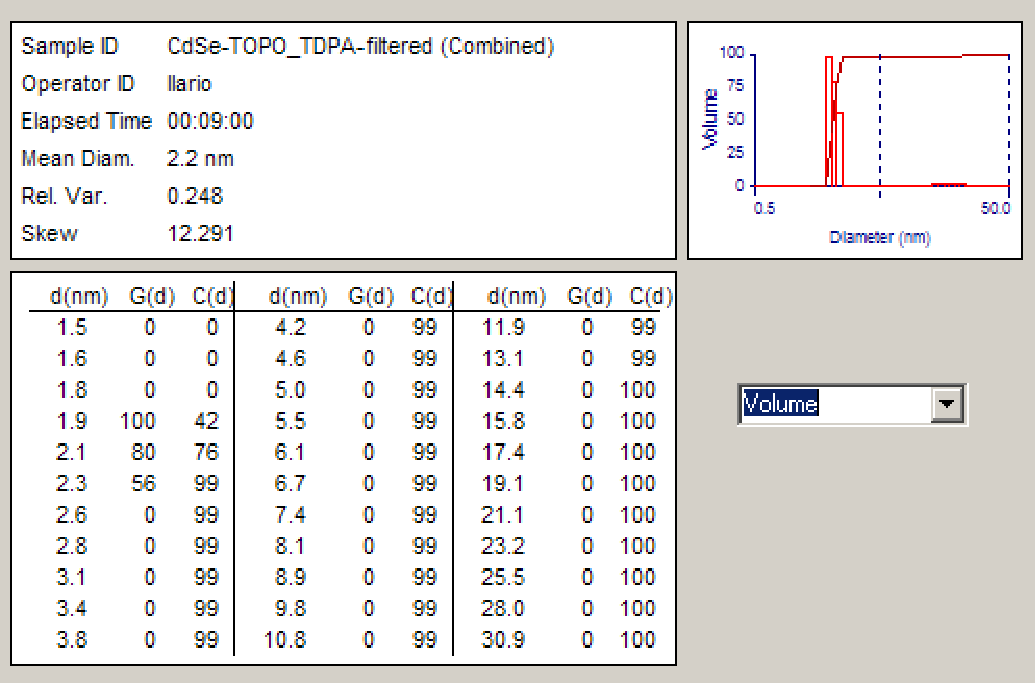
\includegraphics[width=.49\textwidth]{Immagini_Tesi/caratterizzazione/AKT146-TOPOCdSefilter-20100512-msd_summary.pdf}
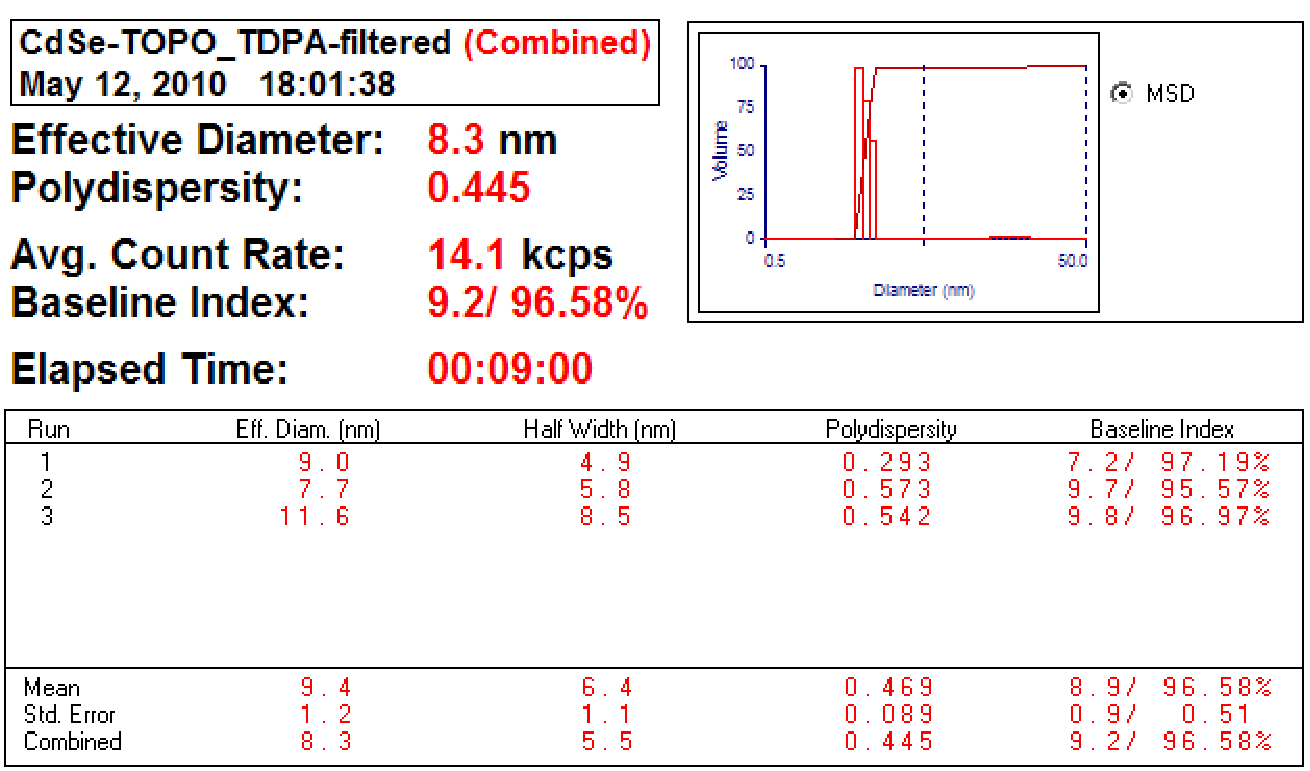
\includegraphics[width=.49\textwidth]{Immagini_Tesi/caratterizzazione/AKT146-TOPOCdSefilter-20100512-totale.pdf}\\
\makebox{\parbox[b]{.495\textwidth}{\centering{(a)}}}
\makebox{\parbox[b]{.495\textwidth}{\centering{(b)}}}
}
\caption{\footnotesize{(a) Media pesata sul volume di NPs di CdSe passivate con TOPO e TDPA in toluene (2.2~nm). \\(b) Media pesata sull'intensità del segnale e qualità del risultato (9.2/10).}}
\label{fig:AKT146-TOPO.CdSefilter-20100512}
\end{figure}

Nello spettro $^{31}$P \{$^1$H\} NMR in~\ref{fig:CdSe-TOPO_TDPA-P_NMR} si può riconoscere il segnale del fosforo legato alla nanoparticella a causa della sua caratteristica larghezza provocata {
dallo scambio tra la soluzione e l'ambiente non omogeneo vicino alla superficie della particella \cite{lig-CdSe-P}. Questo picco allargato può essere assegnato al TOPO \cite{lig-CdSe-P}. Non si osserva un secondo picco allargato per il TDPA perché quest'ultimo, avendo una interazione più forte con la superficie \cite{lig-CdSe-P}, non scambia con la soluzione e non è quindi possibile osservarlo (si trova costantemente in un ambiente quasi solido non analizzabile con tecniche convenzionali di NMR in soluzione).}

I picchi più stretti a $\delta$ 56.23, 44.54, 33.34~ppm sono da assegnare a nuclei di fosforo non legati alla superficie. Il picco a 56.23~ppm si può assegnare a TOPO libero ed il picco a 44.54~ppm può essere assegnato a acido P,P-diottil-fosfinico presente come impurezza nel TOPO commerciale e legante più debole di TOPO~\cite{lig-CdSe-P}.
\begin{figure}
\centering{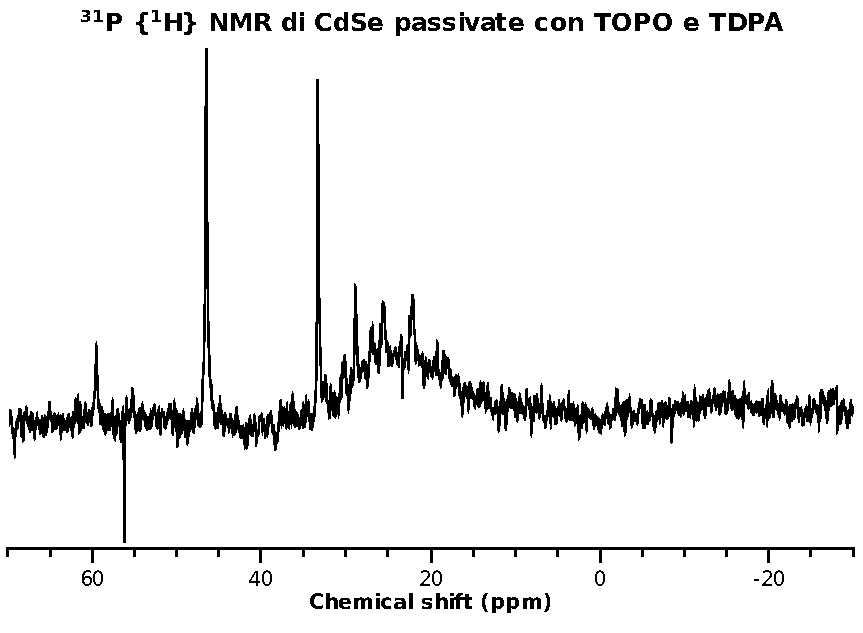
\includegraphics[width=.6\textwidth]{Immagini_Tesi/caratterizzazione/CdSe-TOPO_TDPA-P_NMR.pdf}}
\caption{\footnotesize{Lo spettro $^{31}$P \{$^1$H\} NMR di CdSe con TOPO e TDPA in CDCl$_3$ con una accumulazione di 16 ore (7345 transienti).}
\label{fig:CdSe-TOPO_TDPA-P_NMR}}
\end{figure}

{
In~\ref{fig:CdSe-TEM}-(a) è riportato un dettaglio dell'immagine registrata al microscopio ottico a trasmissione TEM\@. Da una analisi effettuata tramite apposito software si può vedere che le nanoparticelle sono monodisperse ed hanno una dimensione compresa tra 4.0~nm e 4.7~nm.

}
\begin{figure}[!htb]
\centering{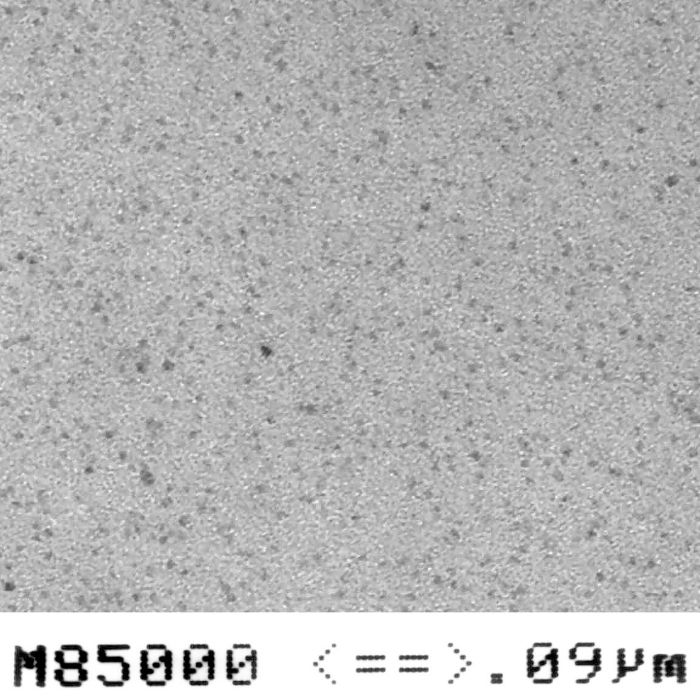
\includegraphics[width=.31\textwidth]{Immagini_Tesi/caratterizzazione/CdSe-TOPO_TDPA-TEM.jpg}
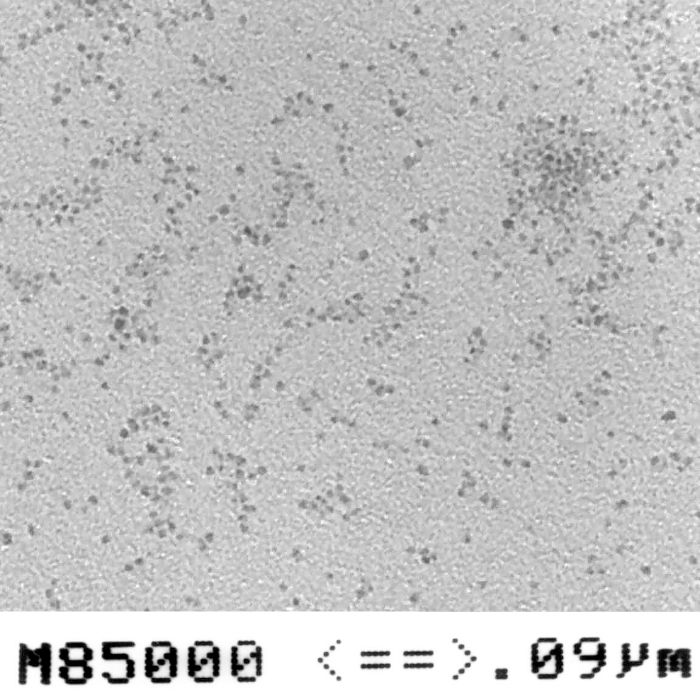
\includegraphics[width=.31\textwidth]{Immagini_Tesi/caratterizzazione/CdSe-pyr-TEM.jpg}
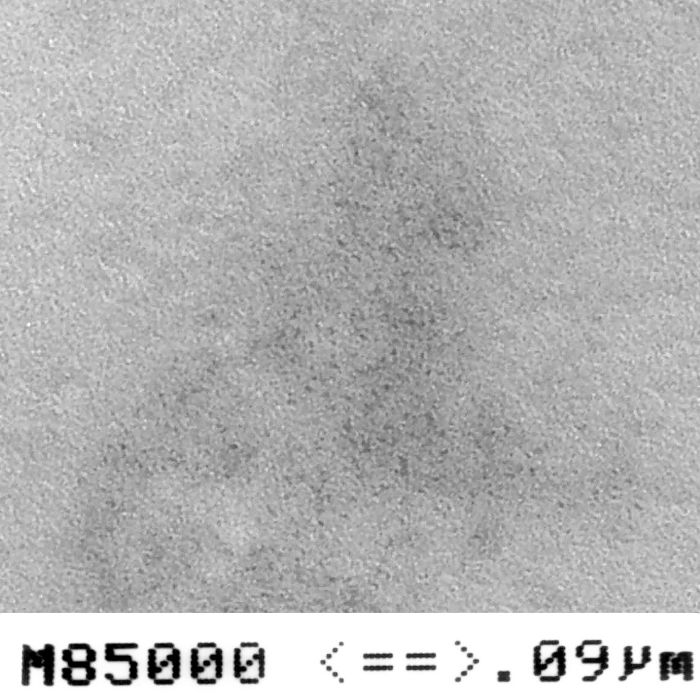
\includegraphics[width=.31\textwidth]{Immagini_Tesi/caratterizzazione/CdSe-P3HT-TEM.jpg}\\
\makebox{\parbox[b]{.31\textwidth}{\centering{(a)}}}
\makebox{\parbox[b]{.31\textwidth}{\centering{(b)}}}
\makebox{\parbox[b]{.31\textwidth}{\centering{(c)}}}}
\caption{\footnotesize{Immagine registrata al microscopio elettronico a trasmissione TEM di NPs di CdSe con: (a) TOPO e TDPA, (b) piridina, (c) polimero {\bf 7}. }}
\label{fig:CdSe-TEM}
\end{figure}
\section{Polimero coniugato}

Qui sono riportati i risultati della caratterizzazione $^1$H-NMR 
effettuata sul poli(3-esiltiofene) regioregolare terminato allile/Br \n{3}. 
\begin{figure}
\centering{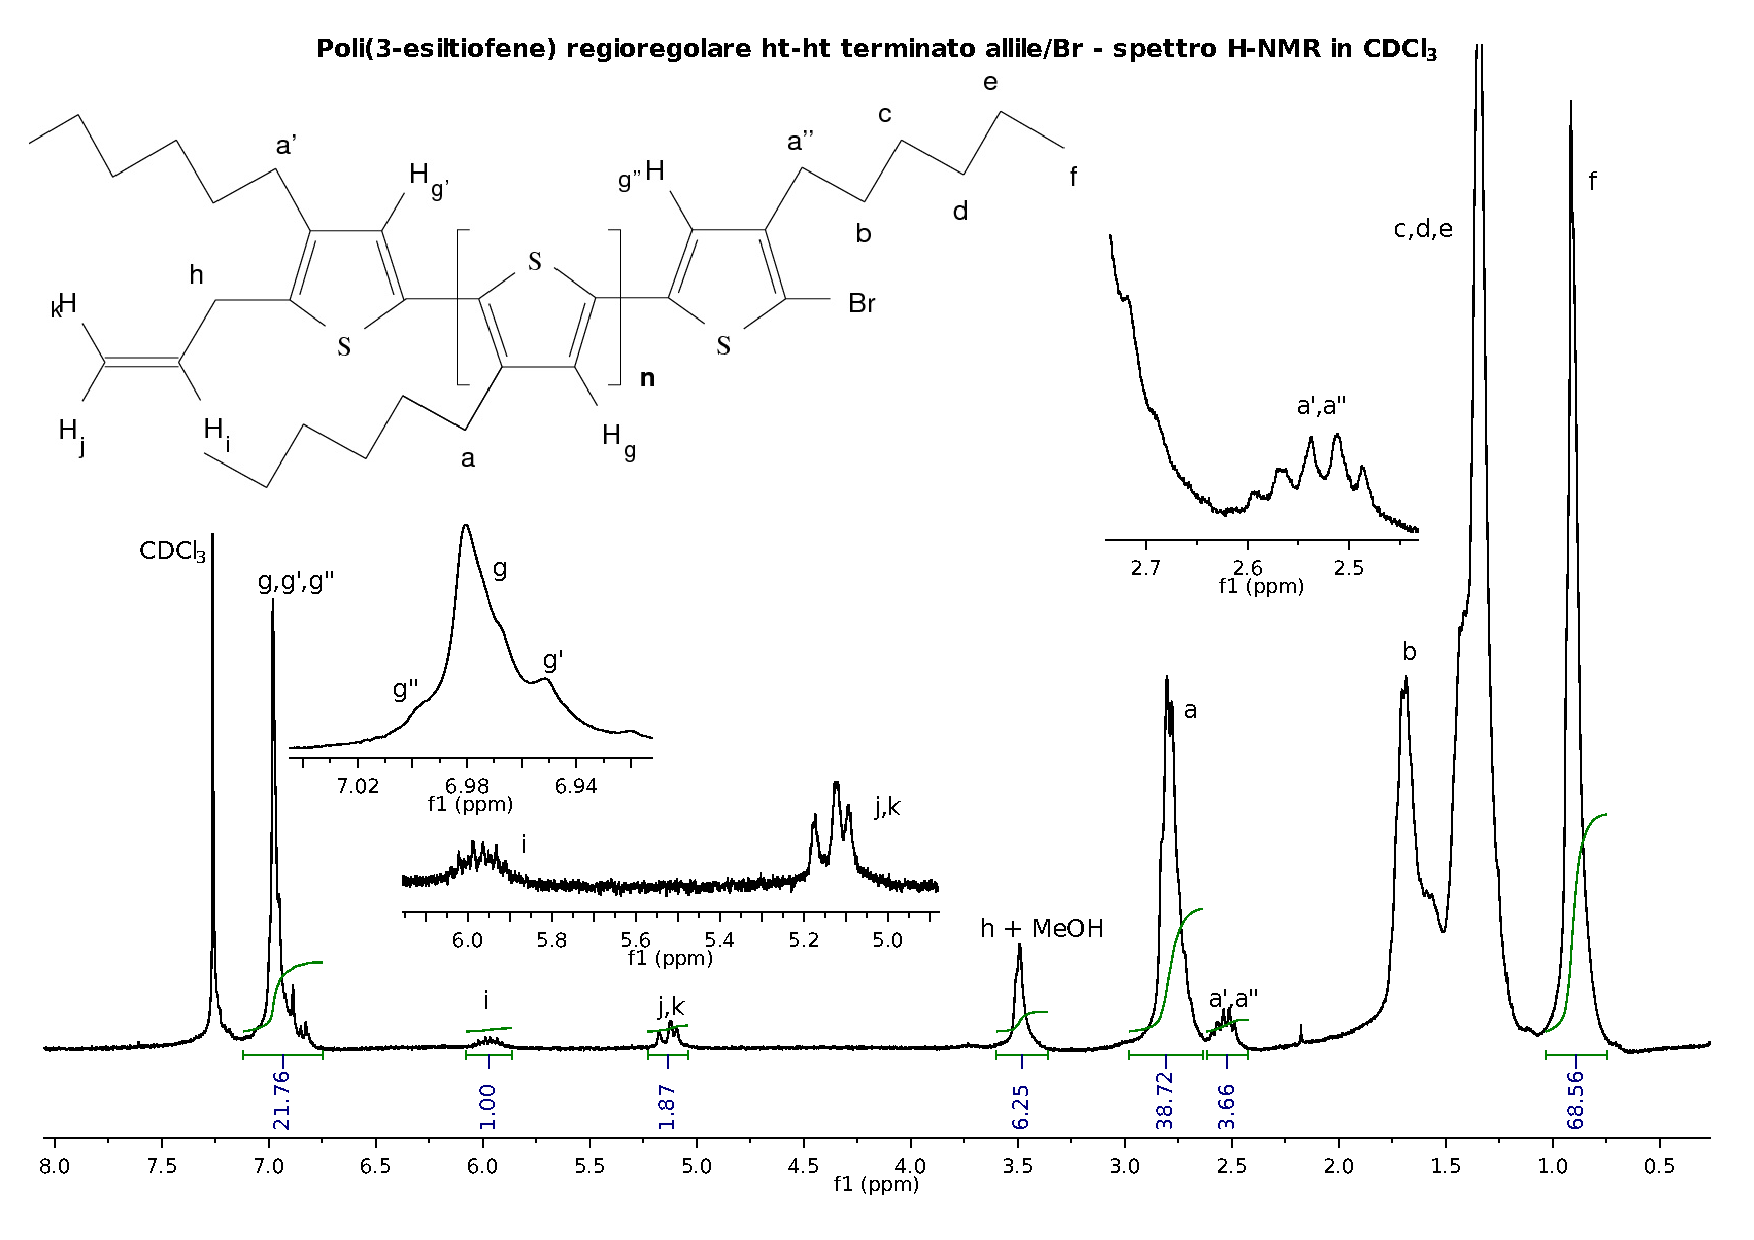
\includegraphics[width=.93\textwidth]{Immagini_Tesi/caratterizzazione/P3HT-HNMR.pdf}}
\caption{\footnotesize{Lo spettro $^1$H-NMR di poli(3-esiltiofene) regioregolare \emph{ht-ht} terminato allile/Br \n{3} in CDCl$_3$, 300MHz.}
\label{fig:P3HT-HNMR}}
\end{figure}

Dallo spettro $^1$H-NMR possiamo ottenere due importanti conferme: la conferma che il nostro polimero è regioregolare \emph{ht-ht} (vedi pagina \pageref{regio-htht}) e che sia monoterminato.

Il picco a 6.98~ppm viene attribuito al protone in posizione 4 sull'anello tiofenico. Questo può trovarsi in 4 distinti ambienti: \emph{ht-ht}, \emph{tt-ht}, \emph{ht-hh} e \emph{tt-hh} dando segnali a diversi \emph{chemical shifts}. Il picco a 6.98~ppm è riportato essere proprio del poli(3-esiltiofene) regioregolare \emph{head-tail-head-tail}~\cite{pol-p3ht-regio}. I \emph{chemical shifts} riportati per le altre regioregolarità sono: \emph{tail-tail-head-tail} 7.00, \emph{head-tail-head-head} 7.02 e \emph{tail-tail-head-head} 7.05~ppm.

Il picco a 2.80~ppm è proprio degli idrogeni {\bf a}, {\bf a'} e {\bf a''} sulla catena alifatica in posizione 3 sul tiofene. I protoni sulle 2 terminazioni danno tripletti, ma a \emph{chemical shift} leggermente diverso dal resto della catena.  Infatti si osservano i 2 tripletti isolati a 2.55~ppm. I tripletti non sono esattamente sovrapposti e danno forma ad un multipletto, questo conferma che {\bf a'} e {\bf a''} si trovano in ambienti diversi, perciò la terminazione è asimmetrica (la terminazione è l'unica differenza nel loro intorno, si ricordi da pagina \pageref{tail-tail} che entrambi i monomeri terminali sono legati al polimero col lato \emph{tail}).

Inoltre osservando le aree integrate e conoscendo l'assegnazione è possibile stimare la lunghezza del polimero. Il risultato di una tale stima è un polimero composto mediamente di 23 unità tiofeniche. 

\section{Modificazione della terminazione}
In questa sezione si riporta la caratterizzazione 
 del poli(3-esiltiofene) terminato allile/legante fosfonico protetto \n{6} ($^1$H-NMR, $^{13}$C-NMR, $^{31}$P NMR con disaccoppiamento protonico e NMR 2 bimensionale HMQC) e del poli(3-esiltiofene) terminato allile/legante fosfonico \n{7} (FT-IR, UV-vis, fotoluminescenza, $^1$H-NMR, $^{13}$C-NMR e $^{31}$P \{$^1$H\} NMR).

\begin{figure}
\centering{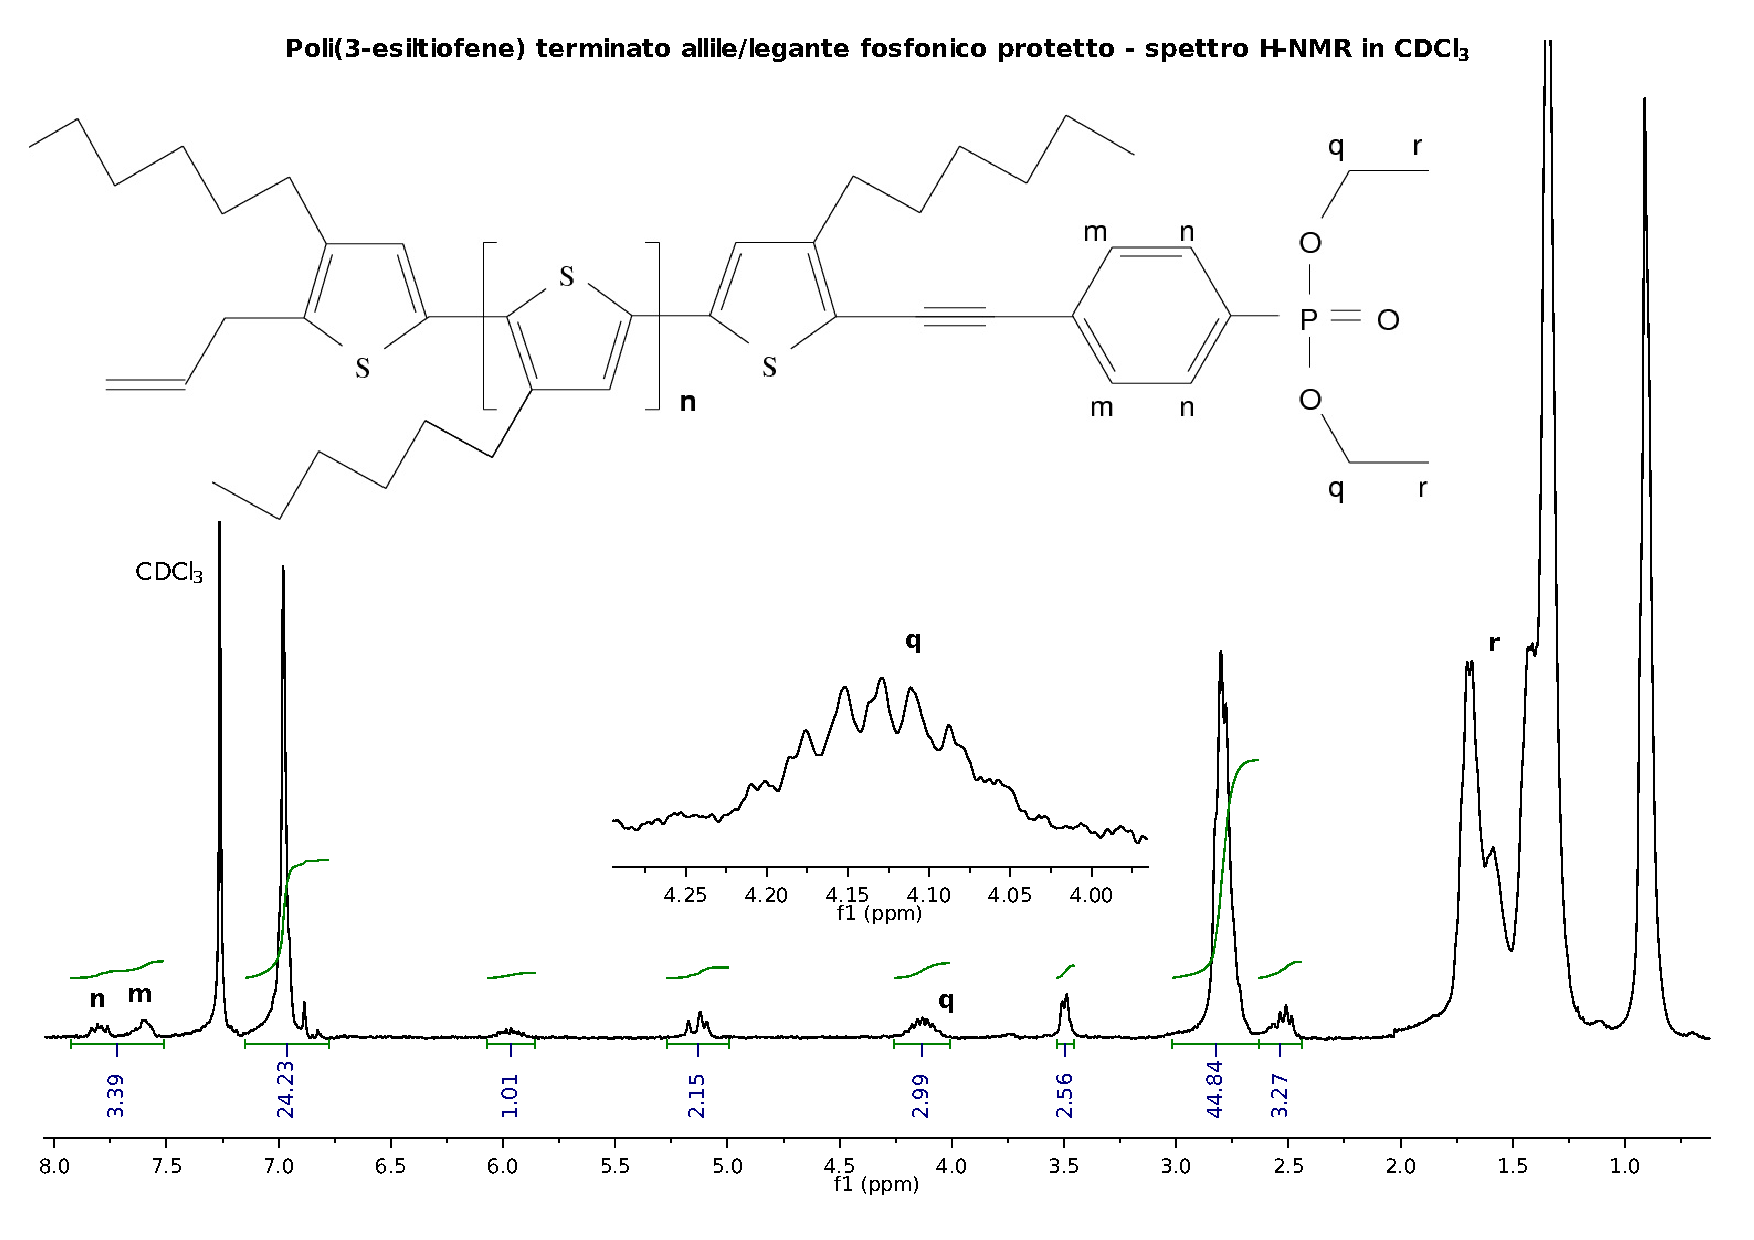
\includegraphics[width=.92\textwidth]{Immagini_Tesi/caratterizzazione/P3HT-leg-HNMR.pdf}}
\vspace{-15pt}
\caption{\footnotesize{Lo spettro $^1$H-NMR di poli(3-esiltiofene) terminato allile/legate fosfonico protetto in CDCl$_3$, 300MHz.}
\label{fig:P3HT-leg-HNMR}}
\end{figure}
Dallo spettro $^1$H-NMR di {\bf 6} riportato in~\ref{fig:P3HT-leg-HNMR} si possono osservare i picchi dell'anello benzenico e delle protezioni etile sul gruppo fosfato. L'area di questi picchi è circa 3 volte l'area corrispondente ad un singolo nucleo di H per una catena di circa 23 unità tiofeniche (sulla base dell'integrale della risonanza a 6.98~ppm) perciò la reazione ha avuto una buona resa ma non una resa quantitativa ed è presente del polimero {\bf 3} (che non viene rimosso dalle purificazioni effettuate). 

È stato registrato anche lo spettro $^{13}$C-NMR di {\bf 6} (75 MHz, \ce{CDCl3})  {
  riportato in~\ref{fig:P3HT-leg-CNMR}. I picchi sullo spettro $^{13}$C-NMR sono stati assegnati grazie all'ausilio di uno spettro bidimensionale HMQC di correlazione tra $^1$H e $^{13}$C direttamente legati. Questo spettro mostra i seguenti picchi: ($\delta_H$ - -  $\delta_C$, \ce{CDCl3}) 0.91 - - 14.0; 1.34 - - 31.9;  1.42 - - 22.9; 1.65 - - 30.8; 2.80 - - 29.6; 6.98 - - 128.8; 7.7~ppm - - 133.0~ppm. }
\begin{figure}
\centering{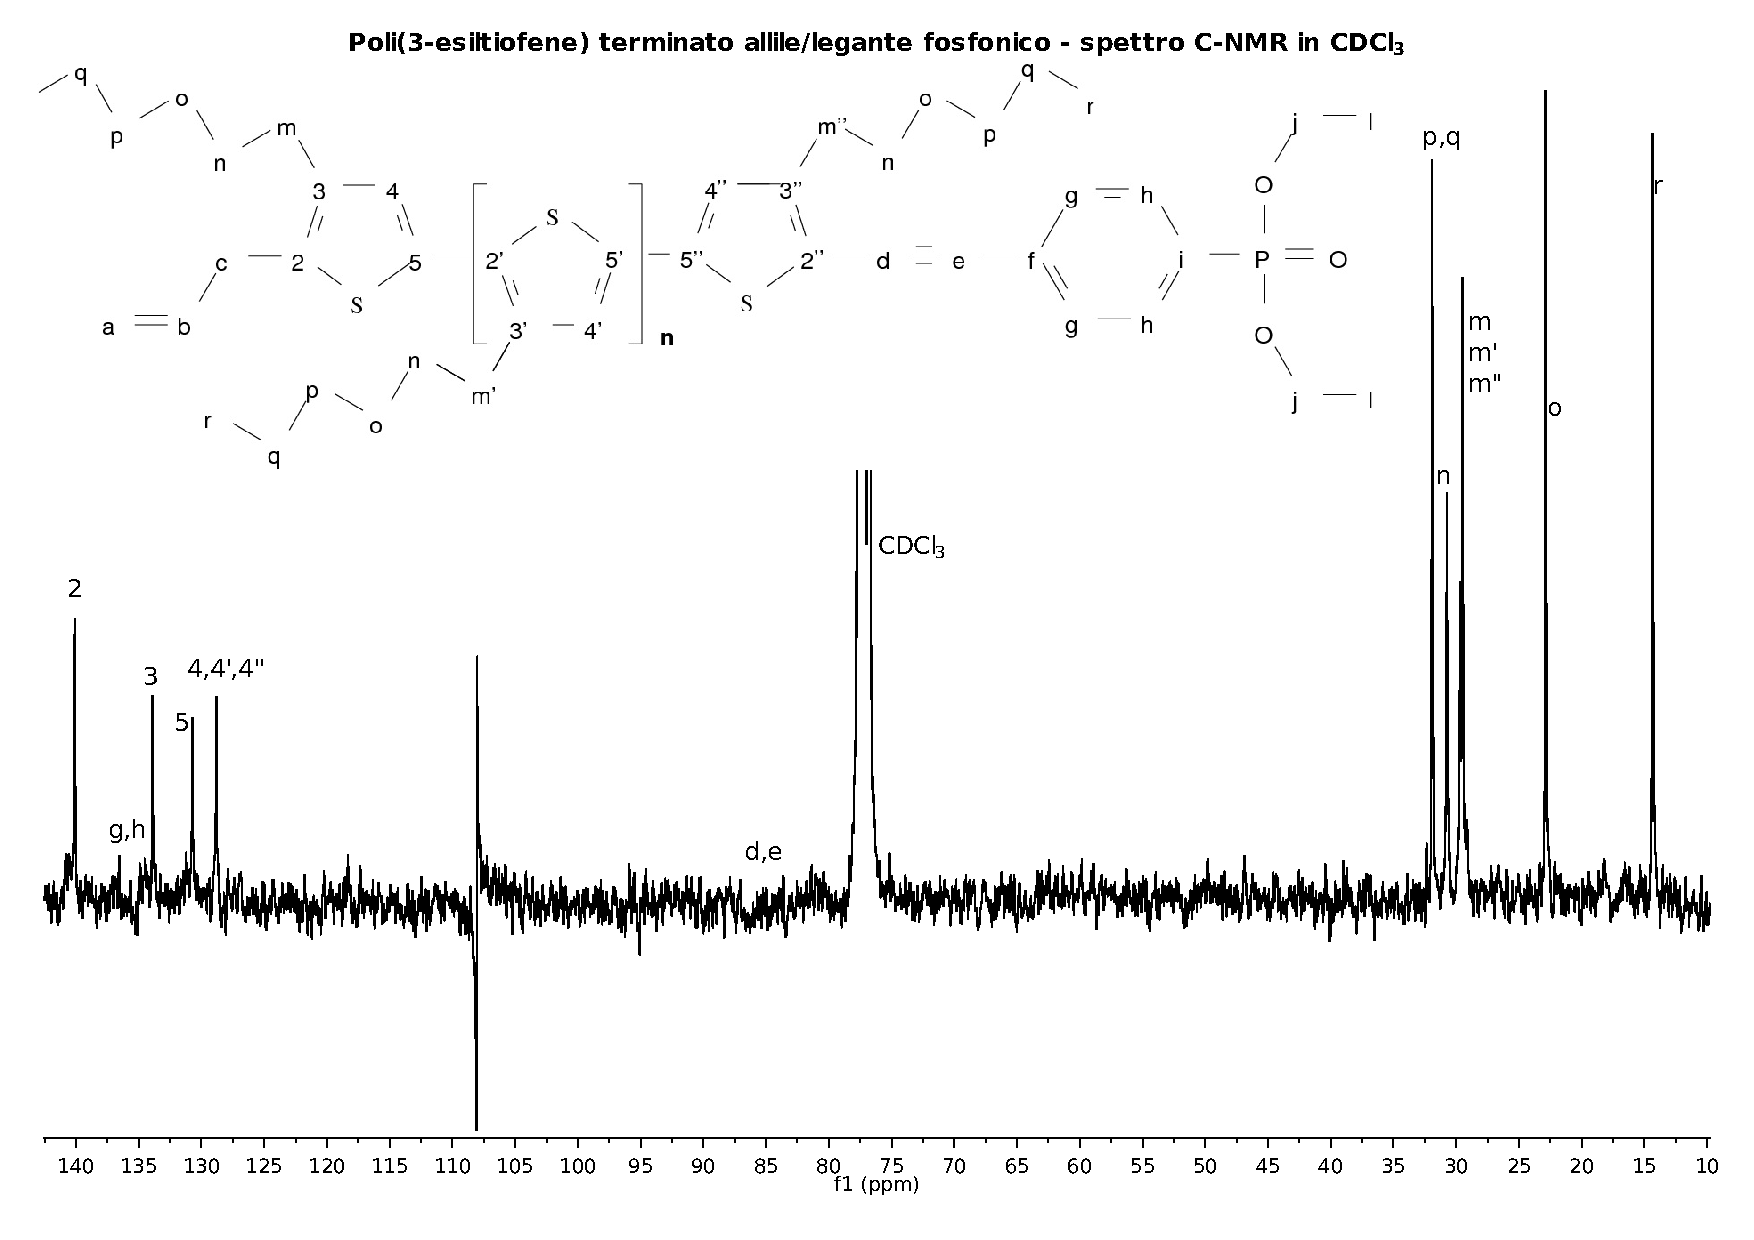
\includegraphics[width=.99\textwidth]{Immagini_Tesi/caratterizzazione/P3HT-leg-CNMR.pdf}}
\caption{\footnotesize{Lo spettro $^{13}$C-NMR di poli(3-esiltiofene) terminato allile/legate fosfonico protetto in CDCl$_3$, 75MHz.}
\label{fig:P3HT-leg-CNMR}}
\end{figure}

All'analisi $^{31}$P \{$^1$H\} NMR in \ce{CDCl3} è visibile solo il picco stretto a 15.79~ppm {
del fosforo sul gruppo legante. In questo caso non si ha allargamento del picco per formazione di micelle perché questa terminazione non è ancora abbastanza polare da formarne.}



\begin{figure}
\centering{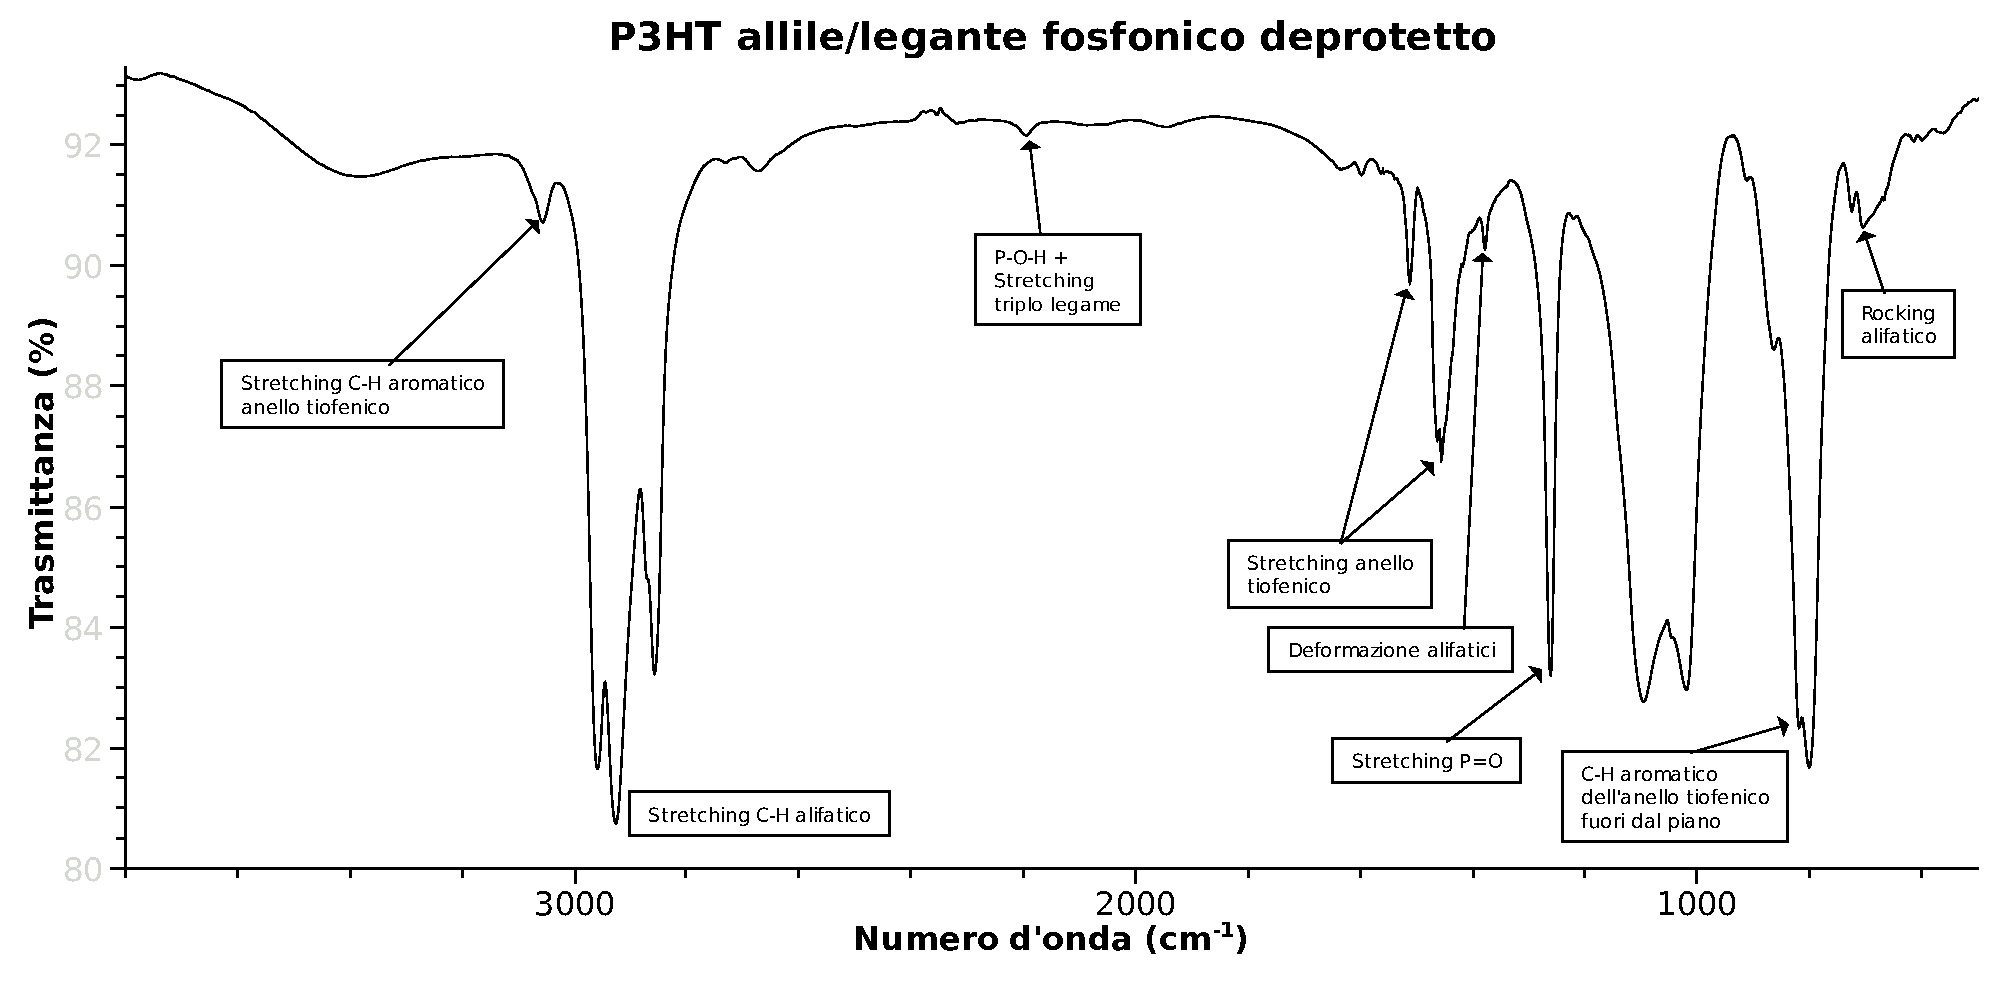
\includegraphics[width=.99\textwidth]{Immagini_Tesi/caratterizzazione/P3HT-leg-deprotetto-IR-assegnato.pdf}}
\caption{\footnotesize{Lo spettro FT-IR di {\bf 7} su pastiglia di KBr.}
\label{fig:P3HT-leg-deprotetto-IR}}
\end{figure}
Nello spettro FT-IR del poli(3-esiltiofene) terminato allile/legante fosfonico \n{7} riportato in~\ref{fig:P3HT-leg-deprotetto-IR} si osserva un piccolo picco a 2195~cm$^{-1}$ attribuibile a {
due segnali sovrapposti: il legame P-O-H del gruppo fosfonico ed il triplo legame presente tra la catena di polimero ed il legante. Più intenso} è il picco attribuibile allo \emph{stretching} P=O a 1262~cm$^{-1}$. Purtroppo gli altri picchi caratteristici del legante vengono coperti dall'assorbimento del polimero, {
ben più intenso a causa della ripetizione dei monomeri risultante in una magnificazione dei loro assorbimenti.}
  


\begin{figure}
\centering{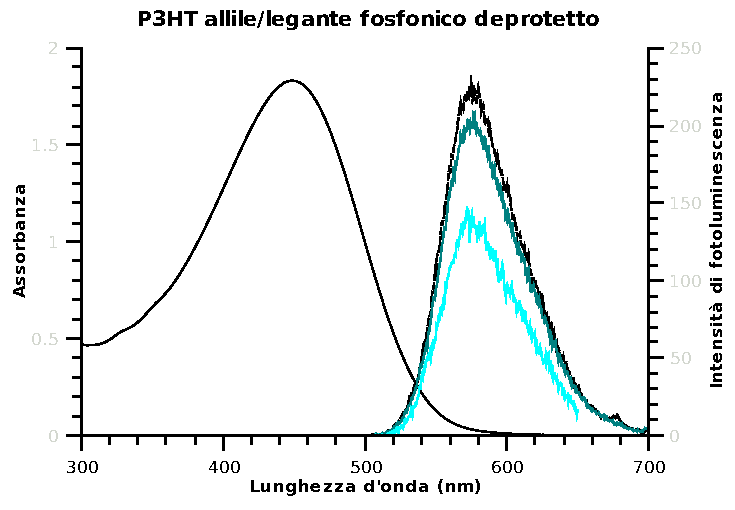
\includegraphics[width=.7\textwidth]{Immagini_Tesi/caratterizzazione/P3HT-leg-deprotetto-UV-PL.pdf}}
\caption{\footnotesize{Spettro di assorbimento ({\bf \large{---}}) e di fotoluminescenza di {\bf 7} in cloroformio a varie lunghezze d'onda: 270~nm ({\Large{{\bf{\color{cyan}---}}}}), 340~nm ({\bf \normalsize{- - -}}), 350~nm ({\Large{{\bf{\color{blue}---}}}}).}
\label{fig:P3HT-leg-deprotetto-UV-PL}}
\end{figure}
Lo spettro di assorbimento UV-vis e lo spettro di fotoluminescenza di {\bf 7} sono riportati in~\ref{fig:P3HT-leg-deprotetto-UV-PL}. Lo spettro UV-vis ha un massimo di assorbimento centrato a 449~nm. In letteratura \cite{pol-p3ht-regio} si trova che per il poli(3-esiltiofene) regiorandom si ha il picco di assorbimento a 428~nm. La posizione del picco a $\lambda$ maggiori indica una maggiore coniugazione che deriva dalla regioregolarità.

Il picco di emissione di fotoluminescenza si trova a 576~nm e non varia in lunghezza d'onda eccitando nell'intervallo tra 270~nm e 400~nm con un massimo in intensità a 341~nm.  

Lo spettro $^1$H-NMR di {\bf 7} differisce dallo spettro di {\bf 6} essenzialmente per la mancanza del multipletto a 4.12~ppm attribuito agli idrogeni metilenici del gruppo etile protezione del gruppo fosfato. Un'altra importante differenza dallo spettro precedente sta nella assenza dei picchi propri degli idrogeni aromatici sul legante. Una possibile giustificazione di questa mancanza sta nella formazione di strutture micellari inverse. Queste si possono formare per la presenza del gruppo legante fosfonico deprotetto polare. Il legante potrebbe quindi trovarsi in una zona con caratteristiche di mobilità ridotta tali da renderlo non osservabile con tecniche convenzionali di NMR in soluzione \cite{lig-micelle-nmr2}. Registrando lo stesso spettro $^1$H-NMR a temperatura maggiore (35°C) non sono state osservate differenze. 

È stato registrato lo spettro $^{13}$C-NMR di {\bf 7}: (75 MHz, \ce{CDCl3}): $\delta$ 1.27, 14.37, 22.90, 29.51, 29.71, 30.75, 31.94, 116.32, 128.81, 130.70, 133.91, 136.54, 140.10~ppm. 

Lo spettro $^{31}$P \{$^1$H\} NMR di {\bf 7} registrato a 40°C è risultato molto diverso dallo spettro di {\bf 6}. Il picco a 15.79~ppm non è più presente mentre si possono osservare dei segnali allargati, tipici {
di una breve permanenza in ambiente liquido con un veloce scambio in un ambiente non uniforme come quello di una struttura micellare \cite{lig-micelle-nmr2}.}
\begin{figure}
\centering{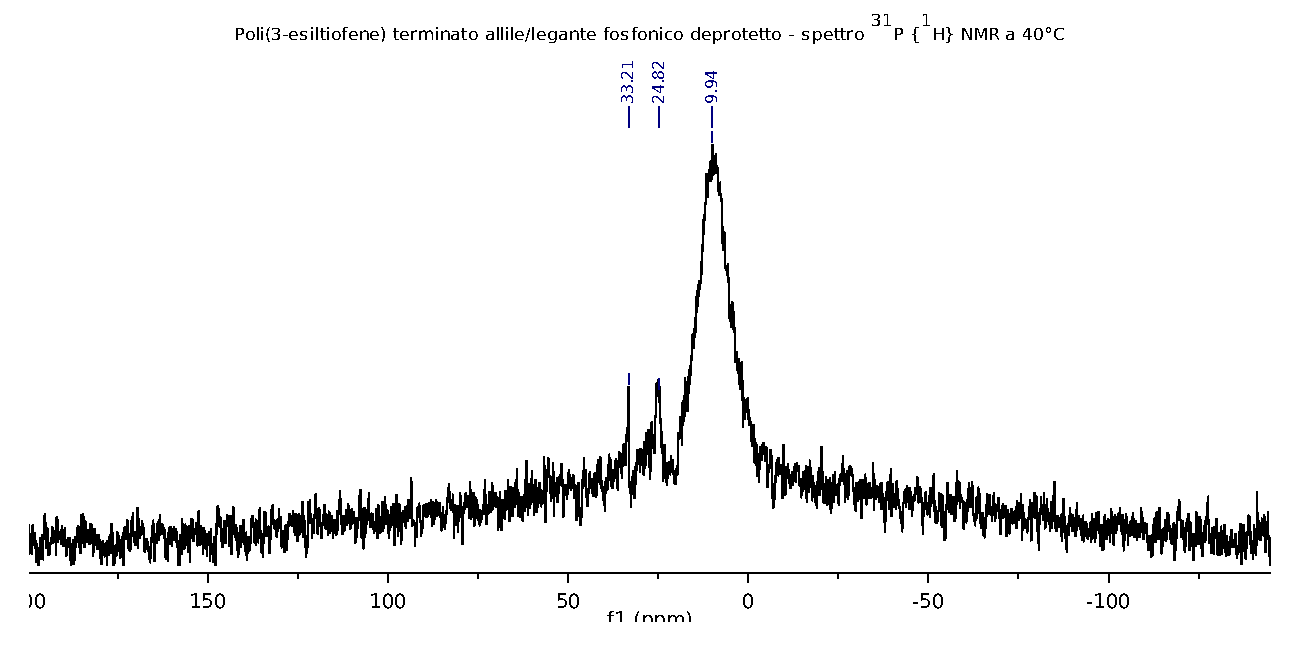
\includegraphics[width=.8\textwidth]{Immagini_Tesi/caratterizzazione/P3HT-leg-PNMR.pdf}}
\caption{\footnotesize{Spettro $^{31}$P \{$^1$H\} NMR di {\bf 7} in \ce{CDCl3} a 40°C con una accumulazione di 18 ore (8624 transienti).}
\label{fig:P3HT-leg-PNMR}}
\end{figure}


\section{Scambio di leganti}

In questa sezione si espongono i risultati della caratterizzazione dello scambio di leganti sulle nanoparticelle (NPs) di CdSe eseguito in successione prima con piridina e poi con il polimero {\bf 7}. 
Del primo prodotto di scambio di leganti sono stati registrati gli spettri FT-IR, UV-vis, fotoluminescenza, $^1$H-NMR, $^{31}$P \{$^1$H\} NMR e TEM\@.  Il prodotto del secondo scambio di leganti è stato caratterizzato registrando gli spettri 
UV-vis, fotoluminescenza, {
  $^{31}$P \{$^1$H\} NMR e TEM.}

Nello spettro FT-IR delle NPs passivate da piridina {
 sono ancora presenti i picchi dovuti alle catene alifatiche di TOPO e di TDPA}.

Lo spettro UV-vis mostra la posizione del primo picco eccitonico a 544~nm.
Questo dato inserito nell'Equazione~\ref{eq:diametro} dà un diametro di 2.9~nm, compatibile col dato ricavato a pagina \pageref{eq:diametro} per le NPs appena sintetizzate. Perciò le particelle non si sono unite a dare aggregati. 

L'analisi di fotoluminescenza sulle nanoparticelle passivate con piridina ha dato un solo picco allargato ed estremamente debole a 555~nm.

Nello spettro $^1$H-NMR 
sono presenti 3 picchi larghi attribuibili alla piridina ($\delta$ 8.62, 7.68, 2.29~ppm). Il fatto che questi picchi siano allargati testimonia lo scambio di piridina tra la soluzione e un ambiente anisotropico come la superficie di una nanoparticella. Inoltre nello spettro sono visibili i picchi di TOPO e di TDPA ancora presenti in soluzione (che si ritiene quindi possano essere efficacemente rimossi con la successiva purificazione).

Infatti nello spettro $^{31}$P \{$^1$H\} NMR di CdSe passivato con piridina non è visibile, nemmeno dopo 11 ore di accumulazione (5485 transienti),  {
il picco allargato che precedentemente era stato attribuito al TOPO, a indicazione di una efficace e pressoché quantitativa sostituzione di quest'ultimo dalla superficie da parte della piridina.} Lo spettro presenta picchi stretti a $\delta$ 56, 23 e 7~ppm. I primi due possono essere attribuiti \cite{lig-CdSe-P} rispettivamente a TOPO ed a TDPA liberi ossia non legati a nanoparticelle.

{
 Nell'immagine registrata al TEM (\ref{fig:CdSe-TEM}-(b)) si osservano nanoparticelle con dimensioni da 3.0~nm a 5.0~nm. Le particelle non sono monodisperse come nella precedente immagine al TEM ma non si ha nemmeno una evidente formazione di aggregati che risulterebbero come grandi macchie nere dovute alla sovrapposizione di NPs anche lungo l'asse $z$ perpendicolare al piano di osservazione. }

Nello spettro UV-vis del prodotto del secondo scambio di leganti il picco a maggiore lunghezza d'onda è dovuto ai nanocristalli e si trova a 550~nm. Utilizzando l'Equazione~\ref{eq:diametro} si ricava un diametro di 3.0~nm, sostanzialmente invariato dalle precedenti misurazioni, ad ulteriore conferma della sostanziale assenza di aggregazione. È presente inoltre una seconda banda di assorbimento con massimo a 447~nm attribuibile al polimero coniugato. Perciò sostanzialmente lo spettro UV-vis è risultato la somma dei due spettri dei precursori.

Il massimo di emissione di fotoluminescenza cambia {
 leggermente } lunghezza d'onda in funzione della $\lambda$ di eccitazione, risultando inoltre tutt'altro che la somma delle bande di emissione di fluorescenza dei due precursori. È riportata in letteratura \cite{lig-PL-quenching} la diminuzione dell'intensità del picco d'emissione delle nanoparticelle indicativa del minore confinamento quantico, diminuito dal contatto elettrico con il polimero coniugato. {
 Infatti la posizione del picco di emissione (573-581~nm) risulta più simile a quella del polimero (576~nm) che delle NPs passivate con TOPO e TDPA (563~nm)}.

{
Lo spettro $^{31}$P \{$^1$H\} NMR con accumulazione di 14 ore (1745 transienti) mostra due picchi molto stretti a 3.59 ed a -1.08~ppm forse non significativi e nessun picco allargato. Lo spettro $^{31}$P \{$^1$H\} NMR registrato a 35°C non presenta significative differenze. L'assenza del picco largo presente nello spettro di {\bf 7} (riportato in~\ref{fig:P3HT-leg-PNMR}) è significativa dell'assenza di polimero legante libero di formare micelle (o comunque presente in concentrazione molto minore del campione analizzato di {\bf 7} puro, tanto da risultare sotto la sua concentrazione micellare critica). Perciò tutto (o quasi) il polimero aggiunto si ritiene debba essere legato alle NPs. Inoltre il fatto che non si abbia nessun picco allargato indica l'assenza di uno scambio dinamico sulla superficie della NP ed una permanenza del gruppo legante sulla superficie delle NPs. Infatti quando il gruppo fosfonico si trova nell'ambiente anisotropo quasi solido della superficie non se ne può osservare il segnale \cite{lig-micelle-nmr2}. Se ne conclude che il legame dev'essere forte.}

{
L'immagine registrata con il microscopio elettronico a trasmissione in~\ref{fig:CdSe-TEM}-(c) non è chiara come le precedenti due immagini a causa della presenza del polimero. Ciononostante si può osservare che le nanoparticelle sono disperse nella matrice di polimero e non sono aggregate se non in blocchi di piccola estensione di cui si può solamente intuire la presenza nell'immagine.}


%%%%%%%% Capitolo4 %%%%%%%%
\chapter{Conclusioni}

Gli obiettivi di questo tirocinio di tesi sono stati raggiunti:
\begin{itemize}
 \item sono state sintetizzate e caratterizzate nanoparticelle di CdSe di dimensioni nanoscopiche,
 \item è stato sintetizzato e caratterizzato poli(3-esiltiofene) regioregolare e terminato con singolo gruppo di acido fosfonico,
 \item sono stati eseguiti e caratterizzati due scambi di leganti sulla superficie delle nanoparticelle.
\end{itemize}
Le nanoparticelle sintetizzate sono risultate avere diametro di 3.0~nm e sono state ottenute con la procedura messa a punto da Peng \etal  \cite{qd-CdSe-CdO}, decisamente più sicura per l'operatore rispetto alle procedure alternative. 

Il poli(3-esiltiofene) sintetizzato è risultato regioregolare \emph{head-tail-head-tail} e terminato in modo asimmetrico. Il metodo utilizzato è stato messo a punto da Jeffries-El \etal \cite{pol-p3ht-end} e risulta in una polimerizzazione quasi vivente, perciò con la possibilità di avere polimeri con bassa polidispersità. La lunghezza media ottenuta è stata di 23 monomeri. Lunghezze maggiori non avrebbero effetto sull'ampiezza del \emph{band gap} ma sarebbero preferibili per future applicazioni in celle fotovoltaiche (una maggiore lunghezza diminuirebbe il trasporto intercatena necessario per la collezione delle cariche sugli elettrodi). 

La molecola contenente un acido fosfonico protetto è stata legata con successo ad una sola terminazione del polimero e deprotetta rendendolo così un polimero legante di superficie nei confronti del CdSe.

Sono stati effettuati 2 scambi di leganti sulla superficie delle nanoparticelle: da una trialchil fosfina ossido ed un acido fosfonico a piridina e poi dalla piridina al polimero terminato con un acido fosfonico. Durante questi processi si è riusciti ad evitare l'aggregazione delle nanoparticelle. Nel primo scambio si è ottenuto, non senza difficoltà, di sostituire completamente i leganti precedentemente presenti. Nel secondo scambio di leganti {%\color{red}
 il polimero è stato quantitativamente legato alle nanoparticelle tramite la terminazione legante.}

Un ideale completamento di questo lavoro richiederebbe la realizzazione di una cella reale e la sua caratterizzazione elettrica {
che potrà essere effettuata in futuro grazie alla collaborazione con altri gruppi di ricerca.} 

{L'aspetto di maggiore innovatività di questo lavoro è stato quindi la sintesi e valutazione di un polimero coniugato contenente una terminazione in grado di coordinare tale polimero con la superficie 
di nanoparticelle inorganiche. Per ottenere efficienze energetiche maggiori nel campo del fotovoltaico ibrido molti sono i fattori su cui porre l'attenzione, ma il primo ed attualissimo problema è la realizzazione di una morfologia \emph{bulk heterojunction}. Si intuisce che l'utilizzo di un polimero legante potrebbe favorire notevolmente il mantenimento di una simile morfologia in una condizione di equilibrio. Va peraltro considerato che la scelta tra i possibili gruppi leganti non è di importanza secondaria perché questa terminazione legante dovrà avere il ruolo di contatto elettrico senza agire da barriera o trappola per i portatori di carica. Questo comportamento è difficile da prevedere a priori. In conclusione si rende necessario un grande lavoro di ricerca, ma questo era prevedibile vista la grande complessità del sistema che vogliamo ottimizzare.
}

%%%%%%%%%%%%%%%%%%%%%% Capitolo 4 %%%%%%%%%%%%%%%%%%%%%%
\chapter{Parte sperimentale}

\section{Informazioni generali}
Per le analisi TLC sono state usate lastre di gel di silice Fluka con indicatore di fluorescenza.
Le purificazioni su colonna sono state eseguite con una fase stazionaria di Gel di silice 60 Fluka ed eluente una miscela composta da {\itshape n}-esano e tetraidrofurano in rapporto 60:40.
Gli spettri $^1$H-NMR, $^{13}$C-NMR, $^{31}$P $\{^1H\}$ NMR e 2D HMQC sono stati registrati con spettrometro Varian XL-300 da 300MHz con rotazione fissata su 20Hz.
Gli spettri IR sono stati registrati con uno spettrofotometro Perkin-Elmer Spectrum One depositando il campione in soluzione su una pasticca di KBr e lasciandolo seccare.
Gli spettri UV-vis sono stati realizzati con uno spettrofotometro Perkin-Elmer Lambda 650.
Gli spettri di fotoluminescenza sono stati registrati con uno spettrofotometro Perkin-Elmer LS 55.
Le analisi DLS (\emph{Dynamic Light Scattering}) sono state realizzate con un apparecchio Brookhaven 90plus.
I solventi toluene, piridina (anidrificata con idruro di calcio), cloroformio (anidrificato con solfato di sodio) e tetraidrofurano sono stati lasciati a riflusso per 7 ore al buio e distillati sotto azoto con apparato di Claisen prima dell’uso. Sono stati conservati sotto azoto con setacci molecolari 3A. 
Le filtrazioni sono state effettuate con filtro per siringa Millipore Millex-FG in PTFE (teflon) da 0.2$\mu$m.
Le centrifugazioni sono state eseguite utilizzando una centrifuga ALC 4236.
Ogni apparecchiatura anidra in atmosfera inerte è stata ottenuta con almeno 3 passaggi di gas inerte (azoto o argon), vuoto, riscaldamento con pistola termica.
Le soluzioni sensibili all’aria o all’umidità sono state trasferite utilizzando siringhe ipodermiche tipo Luer-Lock.

\section{Sintesi di \emph{quantum dots} di CdSe passivati con TOPO e TDPA}
In un pallone a 3 colli con agitazione è stata fatta atmosfera inerte di argon. Vi sono stati inseriti ossido di cadmio$_{(s)}$ ( CdO, 0.05123~g, 0.39896~mmol, Aldrich, 99.99\% ), acido 1-tetradecilfosfonico$_{(s)}$ ( TDPA, 0.223~g, 278.37~g/mol, 0.801~mmol, Alfa Aesar, 98\% ) e tri-ottilfosfina ossido$_{(s)}$ ( TOPO, 3.77855~g, 386.63~g/mol, 9.77291~mmol, Aldrich, 99\% ). Si è scaldato con un mantello riscaldante e nel frattempo il pallone è stato posto sotto vuoto da pompa meccanica per eliminare l'ossigeno, successivamente è stata ripristinata l'atmosfera di argon. Raggiunti i 320°C si è dissolto il CdO rossastro e la soluzione è diventata incolore e limpida. Il pallone è stato lasciato raffreddare fino al raggiungimento di 275°C. In un altro pallone sono stati introdotti tri-ottilfosfina$_{(s)}$ scaldato per renderlo liquido ( TOP, 2.4~mL, 0.831~g/mL, 2.0~g, 370.64~g/mol, 5.4~mmol, Aldrich, 90\% ) e selenio$_{(s)}$ ( Se, 0.0418~g, 0.529~mmol, Aldrich, 99.99\%). Questo è stato scaldato a 45°C ed agitato per mantenere una dispersione. Il contenuto del secondo pallone è stato trasferito in una singola rapida iniezione nel primo pallone. La temperatura è calata fino a 250°C ma è poi stata riportata a 270°C. Il riscaldamento è stato mantenuto per 5 minuti dopo i quali è stato lasciato il pallone con la soluzione rosso cupo al buio per alcune ore a temperatura ambiente. Infine la soluzione è stata conservata a -20°C per il successivo scambio di leganti mentre un'aliquota è stata utilizzata per la caratterizzazione.

Le nanoparticelle in quest'ultima aliquota sono state precipitate dall'ambiente di reazione aggiungendo metanolo disareato (Sigma-Aldrich, 99.8\%). Dopo centrifugazione a 3000rpm per 20 minuti il surnatante è risultato incolore perciò è stato scartato e dell'altro metanolo è stato aggiunto disperdendo il solido. La precipitazione è stata ripetuta 3 volte. Il precipitato è stato seccato con un flusso molto lieve di azoto e quindi ridisciolto in toluene distillato allo scopo di eseguire la caratterizzazione. La soluzione rossa (e verde se osservata sotto illuminazione UV) così ottenuta è stata filtrata con filtro da siringa da 0.2$\mu$m. 

Su questa è stata svolta l'analisi UV-vis, di fotoluminescenza, FT-IR e di \emph{Dynamic Light Scattering}. Dopodiché è stato aggiunto metanolo disareato per riprecipitare le nanoparticelle che sono state centrifugate a 3000~rpm per 20 minuti e seccate con flusso di azoto. È stato successivamente aggiunto CDCl$_3$ (Euriso-Top), un buon solvente per le NPs passivate con TOPO e TDPA, e la soluzione è stata filtrata su filtro da siringa. Questo campione è stato analizzato 
al $^{31}$P $\{^1H\}$ NMR ed al microscopio elettronico a trasmissione. 

La successione di solubilizzazioni in diversi solventi e riprecipitazioni non aveva tanto una funzione preparativa (purificazione) ma piuttosto si è resa necessaria per effettuare le diverse caratterizzazioni su una quantità di prodotto iniziale troppo piccola per poter effettuare prelievi ripetuti.


\section{Sintesi di \emph{quantum dots} di CdSe passivati con piridina}
\label{sec:CdSe-Py}
In un tubo Schlenk con atmosfera inerte di argon sono state poste nanoparticelle di CdSe passivate con TOPO e TDPA (1.348g) e piridina distillata (5~mL). La soluzione è stata agitata per 6 ore a 70°C (con tempi e temperature inferiori non sono stati ottenuti prodotti precipitabili in {\itshape n}-esano (Sigma-Aldrich, puriss.) né in alcuni altri solventi nei quali le nanoparticelle possono perdere la passivazione ed aggregarsi non risultando più solubili in MeOH). Con l'aggiunta di abbondante {\itshape n}-esano le NPs sono state precipitate ed il surnatante è stato scartato dopo centrifugazione a 3000~rpm per 20 minuti. Una parte delle NPs sono state disciolte in \ce{CDCl3} e caratterizzate all' $^1$H-NMR\@. Il solido è stato ripreso in poca piridina, riprecipitato in {\itshape n}-esano e centrifugato a 3000~rpm per 20 minuti; questa operazione è stata ripetuta 5 volte. 

Quindi si è registrato uno spettro $^{31}$P \{$^1$H\} NMR\@. Una ulteriore purificazione è stata eseguita aggiungendo poche gocce di cloroformio e toluene (3~mL) e quindi precipitando con {\itshape n}-esano e centrifugando a 4000rpm per 20 minuti. 
I \emph{quantum dots} di CdSe passivati con piridina e TDPA sono stati seccati con un leggero flusso di gas inerte e quindi sciolti in piridina (0.5~mL) e cloroformio (4.5~mL). Dopo ultrasonicazione per 5 minuti con sonda a ultrasuoni la soluzione è stata centrifugata per 20 minuti a 3000~rpm. Il surnatante è stato filtrato su filtro per siringa da 0.2$\mu$m. 

Questa frazione essiccata è stata ridisciolta in \ce{CDCl3} e caratterizzata all' $^1$H-NMR, al $^{31}$P \{$^1$H\} NMR, all'FT-IR, all'UV-vis ed alla fotoluminescenza. È stata registrata anche una immagine al microscopio elettronico a trasmissione.
\section{Sintesi di poli(3-esiltiofene) regioregolare terminato allile/Br (3)}

In un pallone a tre colli protetto dalla luce è stata ottenuta, e mantenuta per tutta la procedura, l'atmosfera inerte di azoto. Vi è stato versato THF distillato (7~mL) ed il monomero 2,5-dibromo-3-esiltiofene$_{(l)}$ ({\bf{1}}) (1.50~mL, 1.521~g/mL, 2.28~g, 326.09~g/mol, 7.00~mmol) previamente passato all'evaporatore rotante per rimuovere eventuali tracce di solvente. Il pallone è stato posto sotto vuoto da pompa meccanica per eliminare l'eventuale ossigeno disciolto nei liquidi, successivamente è stata ripristinata l'atmosfera di azoto. Utilizzando la siringa ipodermica vi è stato aggiunto il reattivo di Grignard t-butilmagnesio cloruro (7.0~mL, 1.0M in THF, 7.0~mmol, Aldrich). Il pallone è stato lasciato sotto agitazione a 45°C per 4 ore. Una volta raffreddato vi si è aggiunto THF distillato (50~mL) ed il catalizzatore 1,3-bis(difenilfosfino)propano nickel(II) cloruro$_{(s)}$ (0.0630~g, 542.05~g/mol, 0.116~mmol, Aldrich). La soluzione è stata lasciata 20 minuti sotto agitazione al riparo dalla luce. È quindi stato aggiunto allilmagnesio bromuro (1.75~mL, 1.0M in \ce{Et2O}, 
1.75~mmol, Aldrich) ed è agitata la soluzione per 5 minuti. Infine il contenuto del pallone è stato versato goccia a goccia in metanolo (0.75L, Carlo Erba, per analisi) allo scopo di precipitare il polimero formato. La dispersione è stata lasciata sotto agitazione per una notte. 

Il giorno successivo il tutto è stato filtrato attraverso un ditale di cellulosa ed il polimero così raccolto è stato estratto con metanolo e poi con {\itshape n}-esano in Soxhlet fino al termine della colorazione dei solventi uscenti. Il polimero contenuto nel ditale è stato raccolto utilizzando come solvente nell'estrattore Soxhlet del cloroformio distillato. Questa operazione è stata interrotta più volte per sostituire il \ce{CHCl3} contenente il polimero con \ce{CHCl3} distillato. Ciò è stato fatto per minimizzare il danno che può derivare al polimero dal riscaldamento. All'interno del ditale si è osservato il permanere di residuo rosso, probabilmente il catalizzatore. Il polimero ottenuto è stato seccato prima in evaporatore rotante e poi ponendolo sotto vuoto da pompa meccanica. 

Sono stati così ottenuti 0.3897~g di poli(3-esiltiofene) regioregolare \emph{head-tail-head-tail} terminato con un gruppo allile ed un atomo di bromo ({\bf 3}) come solido rosso scuro, con una resa del 33\%.

Una parte del polimero è stata disciolta in \ce{CDCl3} per eseguire la caratterizzazione $^1$H-NMR.



\section{Sintesi del dietil estere dell'acido (4-etinilfenil) fosfonico (5)}
In un tubo Schlenk con atmosfera inerte di azoto è stato versato il catalizzatore \ce{PdCl2(PPh3)2}$_{(s)}$ (0.1329~g, FW=701.90~g/mol, 0.1893~mmol) sciolto in pochi mL di etere dietilico. L'etere dietilico è stato rimosso utilizzando il vuoto da pompa meccanica. È stato aggiunto dietil (4-bromofenil)fosfonato$_{(s)}$ ({\bf 4}) (1.5012~g, 293.09~g/mol, 5.1219~mmol)
, trietilammina (10~mL) e, utilizzando una siringa ipodermica, etiniltrimetil silano$_{(l)}$ (0.83~mL, 0.71~g/mL, 0.59~g, 98.22~g/mol, 6~mmol). 
Infine è stato aggiunto CuI$_{(s)}$ ( 0.0202~g, 190.45~g/mol, 0.1061~mmol) sciolto in trietilammina$_{(l)}$ (5~mL) precedentemente disareato tramite vuoto. È stato collegato il tubo Schlenk alla pompa meccanica da vuoto per eliminare le tracce di ossigeno. Il tutto è stato lasciato sotto agitazione a 90°C per una notte.

La soluzione è stata quindi ridotta di volume utilizzando il vuoto da pompa meccanica. 
È stato aggiunto {\itshape n}-esano e filtrato il surnatante su filtro Gooch di vetro. Il solido rimasto nel tubo Schlenk è stato lavato con una miscela di {\itshape n}-esano  e tetraidrofurano 1:1 fino a decolorazione del solido (fino al persistere della colorazione gialla del catalizzatore). Anche il solvente di lavaggio è stato filtrato su filtro di vetro ed aggiunto alla precedente aliquota filtrata. Da questa soluzione è stato rimosso il solvente all'evaporatore rotante ottenendo un liquido marrone viscoso. Vi è stato aggiunto metanolo anidro (10~mL) e, goccia a goccia, una soluzione acquosa satura di KOH (0.78~g di KOH, 14~mmol, Carlo Erba, per analisi). Il tubo è stato lasciato sotto agitazione protetto dalla luce per 4 ore. La soluzione così ottenuta è stata estratta in imbuto separatore con acqua e \ce{CH2Cl2}. La fase organica è stata anidrificata con solfato di sodio anidro mentre la fase acquosa è stata scartata. Il solvente è stato rimosso utilizzando l'evaporatore rotante. Il legante è stato purificato su colonna impaccata con silice (80~g, Fluka gel di silica 60) utilizzando come eluente una miscela di {\itshape n}-esano  e THF 60:40. Le frazioni raccolte sono state analizzate con TLC\@. Le frazioni in cui si è osservata quasi esclusivamente la macchia del legante fosfonico desiderato sono state unite ed è stato rimosso il solvente con evaporatore rotante. 
 
Sono stati così ottenuti 0.1510~g di legante dietil estere dell'acido (4-etinilfenil) fosfonico ({\bf 5}). Il prodotto è stato conservato in {\itshape n}-esano  a -20°C. 

\section{Sintesi di poli(3-esiltiofene) terminato allile/legante fosfonico protetto (6)}
Il poli(3-esiltiofene) terminato allile/Br \n{3} (0.2g) è stato posto in un tubo Schlenk in cui è stata fatta atmosfera inerte di azoto. È stato aggiunto il legante \n{5} (0.0143~g, 238.22~g/mol, 60.0~$\mu$mol), il catalizzatore \ce{PdCl2(PPh3)2}$_{(s)}$ (0.0040~g, 5.7~$\mu$mol) e tetraidrofurano distillato (9~mL).
La soluzione è stata posta sotto vuoto da pompa meccanica per eliminare gas disciolti.
Infine è stato aggiunto CuI$_{(s)}$ (0.0019~g, 10~$\mu$mol) sciolto in trietilammina$_{(l)}$ (6~mL) precedentemente degassata. Dopo 3 cicli di vuoto azoto il tubo Schlenk è stato lasciato sotto agitazione al riparo dalla luce a 65°C per una notte.

Il polimero è stato quindi precipitato in metanolo e purificato con metanolo in estrattore Soxhlet. Sostituendo il metanolo con \ce{CHCl3} è stato raccolto il polimero {\bf 6}. Nell'eseguire la raccolta in \ce{CHCl3} si è limitato il tempo di permanenza del polimero in cloroformio bollente rimpiazzando più volte il solvente con cloroformio distillato puro. Il prodotto {\bf 6} è stato seccato all'evaporatore rotante e per vuoto da pompa meccanica. Sono stati ottenuti 0.21~g di solido rosso scuro. È stato registrato uno spettro di \n{6} all'FT-IR\@. Una porzione è stata sciolta in \ce{CDCl3} per eseguire la caratterizzazione $^1$H-NMR, $^{13}$C-NMR, $^{31}$P \{$^1$H\} NMR ed HMQC ($^1$H e $^{13}$C NMR bidimensionale). 


\section{Sintesi di poli(3-esiltiofene) terminato allile/legante fosfonico (7)}
Il poli(3-esiltiofene) terminato allile/legante fosfonico protetto \n{6} (0.14g) è stato posto in un tubo Schlenk in atmosfera inerte di azoto e sciolto in \ce{CH2Cl2}$_{(l)}$ (15~mL). Si è aggiunto trietilammina$_{(l)}$ (1.5~mL). Prestando particolare attenzione a minimizzare il contatto con l'aria ed utilizzando una siringa ipodermica è stato versato nel tubo Schlenk trimetilbromosilano$_{(l)}$ (0.5~mL, 1.16~g/mL, 153.09~g/mol, 4~mmol, Aldrich, 97\%). 
Il recipiente è stato lasciato sotto agitazione a temperatura ambiente per una notte. Il giorno successivo è stato scaldato a riflusso per 2 ore ed è stato trasferito in metanolo (0.3L) per la precipitazione. Il precipitato è stato raccolto filtrando su filtro di carta, recuperato lavando il filtro con cloroformio e seccato all'evaporatore rotante e sotto vuoto da pompa meccanica. Sono stati così ottenuti 0.1738~g di solido rosso contenente impurezze bianche (probabilmente prodotti di reazione del trimetilbromosilano con dell'acqua presente nel metanolo utilizzato). Una porzione è stata sciolta in \ce{CDCl3} ed è stata caratterizzata $^1$H-NMR, $^1$H-NMR a 35°C, $^{13}$C-NMR, $^{31}$P \{$^1$H\} NMR a 40°C. È stato registrato uno spettro FT-IR, uno di assorbimento UV-vis ed un'analisi di fotoluminescenza.

\section[Sintesi di \emph{quantum dots} di CdSe passivati con polimero]{Sintesi di \emph{quantum dots} di CdSe passivati con poli(3-esiltiofene) terminato allile/legante fosfonico}
Al polimero {\bf 7} (0.21g, dei quali una piccola parte ottenuti da una seconda preparazione identica a quella qui riportata) disciolto in cloroformio (0.5~mL) sono state aggiunte le nanoparticelle (0.183g) ottenute nella Sezione~\ref{sec:CdSe-Py} seccate e ridisciolte in cloroformio (1~mL). La soluzione così ottenuta è stata lasciata a temperatura ambiente per 2 giorni. Questo prodotto è stato caratterizzato con FT-IR, UV-vis, fotoluminescenza, TEM e $^{31}$P \{$^1$H\} NMR.

%%%%%%%%%%%%%%%%%%%% Bibliografia %%%%%%%%%%%%%%%%%%%%%%
\bibliographystyle{unsrt}
\bibliography{tesi.bib}
\end{document}
